% !TEX encoding = UTF-8 Unicode
\documentclass[a4paper, 12pt]{article}

\usepackage[margin=3cm, left=3cm, right=3cm, top=3cm, bottom=3cm]{geometry}
\usepackage[boldfont]{xeCJK}
\usepackage{fontspec}
\usepackage{type1cm}
%\usepackage{txfonts}
\usepackage{indentfirst}
\usepackage{titlesec}
\usepackage{titletoc}
\usepackage{xCJKnumb}
\usepackage{setspace}


% reference
\usepackage{cite}

% image and table title
\usepackage{caption}
\usepackage{subcaption}

%\usepackage{booktabs}
\usepackage{listings}
\lstset{xleftmargin=0.1cm, xrightmargin=0.1cm}

% image
\usepackage{graphicx}
\usepackage{pdfpages}

% for pseudo code
\usepackage{algorithm}
\usepackage{algpseudocode}
\usepackage{amsmath}

% for reference website url
\usepackage{url}

% for water mark
\usepackage{wallpaper}

% for table
\usepackage{multirow}
\usepackage{array}

\bibliographystyle{unsrt}

\setmainfont{Times New Roman}

\XeTeXlinebreaklocale "zh"

\setCJKfamilyfont{xxm}{PMingLiU}

\linespread{1.5}

\titlecontents{section}[0em]{\fontsize{13}{18}}{第\,\xCJKnumber{\thecontentslabel}\,章\,\quad}{}{\titlerule*[1ex]{.}\contentspage}
\titlecontents{subsection}[2em]{\fontsize{11}{16}}{\thecontentslabel\,\quad}{}{\titlerule*[1ex]{.}\contentspage}

\renewcommand{\figurename}{圖}
\renewcommand{\tablename}{表}
\newcommand{\loflabel}{圖}
\newcommand{\lotlabel}{表}
\titleformat{\section}{\centering\fontsize{14}{21}\bfseries}{第\,\xCJKnumber{\thesection}\,章}{1em}{}
\titleformat*{\subsection}{\fontsize{12}{18}\bfseries}

\begin{document}

\includepdf[pages={1,2}]{cover_v1.pdf} 
\pagenumbering{Roman}
\addcontentsline{toc}{section}{摘要}
\begin{center}

\large{基於Apache Spark 建構串流 XML Veracity 真實度之模型}\\
\vspace{0.83cm}

\makebox[3cm][r]{\large{學生:}}
\makebox[3cm][l]{\large{紀承甫}}
\hfill
\makebox[3cm][r]{\large{指導教授:}}
\makebox[3cm][l]{\large{陳世穎}}
\vspace{0.83cm}
\\
\large{國立臺中科技大學}\large{ 資訊工程系}
\vspace{0.83cm}
\renewcommand{\abstractname}{摘要}
\begin{abstract}
%近幾年大數據的數據量飛快地成長,超過TB等級的數據已是隨處可見。而數據傳輸在大數據中是一個重點探討的問題,大數據在做資料交換的時候,由於資料量龐大,所以資料的真實度不易掌控,也就是大數據5V當中的Veracity是我們最關切的問題。\\\par
%而XML(延伸標記語言 eXtensible Markup Language)作為現今通用的網路資料交換格式,隨著網際網路資料的增長,也已經同樣具有大數據(Big Data)的特徵。在近幾年來,產業界與學界都將大數據列為重要研究議題,並投入相當多的資源支持大數據的研究。\\\par
%本研究提出使用Apache Spark建構串流XML Veracity真實度模型以及真實度模型應用程式開發介面(Veracity Model Application Programming Interface, Veracity Model API),來解決大數據在資料傳輸當中我們所關心的真實度Veracity的問題,並可以讓使用者知道文件有多少可信度。XML真實度模型計分是一個給定一個被量測XML文件,讓模型進行被量測XML文件與標準XML文件的比較,並給定一個量化分數的系統。本研究建構一個利用Apache Spark 的平行化處理,加速真實度模型整體的運算速遞及效能的模組。讓使用者進行串流的XML文件上傳,再將上傳文件放入由Apache Spark建構的真實度計分模型來進行真實度計分,XML文件真實度有很多面向可以做詮釋。本研究設計一個基於物件導向程式設計的真實度模型,藉由物件導向的特性,設計抽象類別來建構一個真實度的維度$(Dimension\ i, D_i)$,再讓使用者繼承此類別實作模型的功能。換言之就是讓使用者決定需要有什麼樣的屬性$(Attribute\ j, A_{i, j})$才可以評價真實度,以及需要有什麼樣的量化和計分方式才可以將真實度呈現出來。如此這個模型的設計將具有彈性且有助於使用者在面對大量XML資料的時候能夠有一個真實度計分的量化標準。在未來開發大數據應用的時候,可以對於在傳輸資料的時候有一個依據來知道資料的可靠程度。
近年大數據的數量飛速成長,而龐大的數據會產生大量的應用。每一個應用都會產生資料交換,XML (eXtensible Markup Language)作為現今通用的網路資料交換格式,隨著網際網路資料的增長,也已經同樣具有大數據(Big Data)的特徵。本研究建構XML真實度模型應用程式開發介面(XML Veracity Model API)來解決大數據在資料傳輸中真實度不易量化的問題。XML文件真實度基於資料理解性有很多面向可以做詮釋,使用真實度模型API,使用者可以自行設計自己所認為的文件真實度的維度以及屬性,並產生量化的分數。且為了因應現今串流資料應用的增加,且又因串流XML資料又有結構上的問題,難以驗證真實度。本研究將真實度模型應用到串流資料,並且使用Apache Spark 增加模型的處理效能,來達到快速處理串流XML的目的,以及驗證真實度模型的設計架構。\\
\vspace{1.8em}
\noindent\textbf{關鍵字}:巨量資料、XML、串流、Apache Spark、真實度
\end{abstract}

\end{center}
\newpage

\addcontentsline{toc}{section}{Abstract}
\begin{center}

\large{Streaming XML Veracity Model Based on Apache Spark}\\
\vspace{0.83cm}

\makebox[3cm][r]{\large{Student:}}
\makebox[3cm][l]{\large{Cheng-Fu Ji}}
\hfill
\makebox[3cm][r]{\large{Advisor:}}
\makebox[3cm][l]{\large{Shin-Ying Chen}}
\vspace{0.83cm}
\\
\large{Department of computer Science and Information Engineering}\\
\large{National Taichung University of Science and Technology}
\vspace{0.83cm}
\renewcommand{\abstractname}{Abstract}

\begin{abstract}
In recent years, the volume of data contained by the big data has increased rapidly, and huge data will generate a lot of applications. Every application generates data exchange. XML (Extensible Markup Language) is a common network data exchange format. With the growth of Internet data, it also has the characteristics of big data. This study constructs the XML Veracity application development interface (XML Veracity Model API) to solve the problem that the realism of big data is not easy to quantify in data transmission. The truth of XML file is based on data understandability and can be interpreted and used. Veracity Model API, users can design their own dimensions and attributes of document realism and generate quantified scores. In order to respond to the increase in the application of streaming data today, and because of the structural problems of streaming XML data, it is difficult to verify the realism. This study applies the Veracity model to streaming data and uses Apache Spark to increase the processing performance of the model to achieve the purpose of quickly processing streaming XML and verifying the design architecture of the realism model.\\
\vspace{1.8em}
\noindent\textbf{Keywords}:Big Data, XML, Streaming, Apache Spark, Veracity
\end{abstract}

\end{center}
\newpage


\begin{center}
\renewcommand{\contentsname}{目錄}
\addcontentsline{toc}{section}{目錄}
\tableofcontents
\end{center}
\newpage

\begin{center}
\renewcommand{\listtablename}{表目錄}
\renewcommand{\numberline}[1]{\fontsize{13}{19}{\lotlabel~#1}\hspace*{1em}}
\addcontentsline{toc}{section}{表目錄}
\listoftables
\end{center}
\newpage

\begin{center}
\renewcommand{\listfigurename}{圖目錄}
\renewcommand{\numberline}[1]{\fontsize{13}{19}{\loflabel~#1}\hspace*{1em}}
\addcontentsline{toc}{section}{圖目錄}
\listoffigures
\end{center}
\newpage

\setcounter{page}{1}
\pagenumbering{arabic}

\begin{spacing}{1.5}

\begin{center}
\section{緒論}
\end{center}

\subsection{背景}
近年來數據以飛快的速度成長,TB或是PB等級的數據隨處可見。在這資料快速產生且數據快速交換的時代,大數據一詞也常被提及。國際數據公司(International Data Corporation, IDC)有研究指出\cite{gantz2011extracting},在2011年,創建和複製的資訊量以及資料量將超過1.8 ZB。這麼龐大的資料也成了產業界與學術界所需要探討的重要議題。而有這麼大量的資料也意味著會有大量的應用產生,而這一些應用當中一定會需要資料的交換,而在交換資料的時候,大多數的應用會選擇XML。\\\par
在大數據中常使用5V\cite{ibm5v}\cite{khan2014big}來描述大數據的特性。所謂的5V是指Volume、Vleocity、Variety,、Value以及Veracity。Volume是指產生的資料量;Velocity是指資料產生的速度;Variety是指資料的多樣性;Value是指資料的價值;Veracity\cite{veracityimpor}是指資料的可信度或是真實度。而大數據在做資料交換的時候我們所關心的是資料的可信度或是真實度,也就是上述所提到的Veracity,這會影響到我們在做資料分析的結果可信度。假使進來的資料不具可信度的話,那麼所分析出來的結果自然也就不具有任何價值。本研究基於Apache Spark建構XML Veacity 真實度模型,利用Apache Spark 分散式大數據處理引擎,來計算並建構大型XML文件的Veracity 模型,並且將此模型應用在串流XML文件的Veracity 真實度評分。

\subsection{XML}
可延伸標記式語言(Extensible Markup Language,簡稱XML)\cite{rfc7303},是一種作為資料交換的結構化資料格式。XML是從標準通用標記式語言(SGML)中簡化修改出來的。XML是從1995年開始有雛形,並向全球資訊網聯盟(World Wide Web Consortium,簡稱W3C)提案,而在1998年2月發布為W3C的標準(XML 1.0)。\\\par
XML的特色在於文件內的標籤名稱可以由使用者自行定義,而XML文件必須是結構完整的(well-formed)。所謂的well-formed是指XML要符合每一個標籤都要有起始元素之巢狀結構,而符合格式規範,如DTD或XML Schema得則稱為有效的XML(Valid XML)。在XML中我們為了確保文件的格式正確性,會使用DTD(Document Type Definition)\cite{dtd}或是XML Schema\cite{xsd}。DTD是XML提供的文件驗證機制,這是用來定義文件合法區塊,也就是定義元素的架構,有使用DTD的XML都必須依照DTD所定義的格式來呈現。圖\ref{xml1}是一個使用DTD且well-formed的XML文件,在圖\ref{xml1}當中的第2行到第8行即是DTD驗證的格式。從第2行開始宣告了這一份XML文件的根節點(root),再來第3行宣告了根節點下有哪一些子節點,第4行到第7行宣告了子節點下皆為資料,沒有接續的子節點。

\begin{figure}[H]
\centering
\graphicspath{{/Users/FUDA/Documents/masterThesis/image/}}
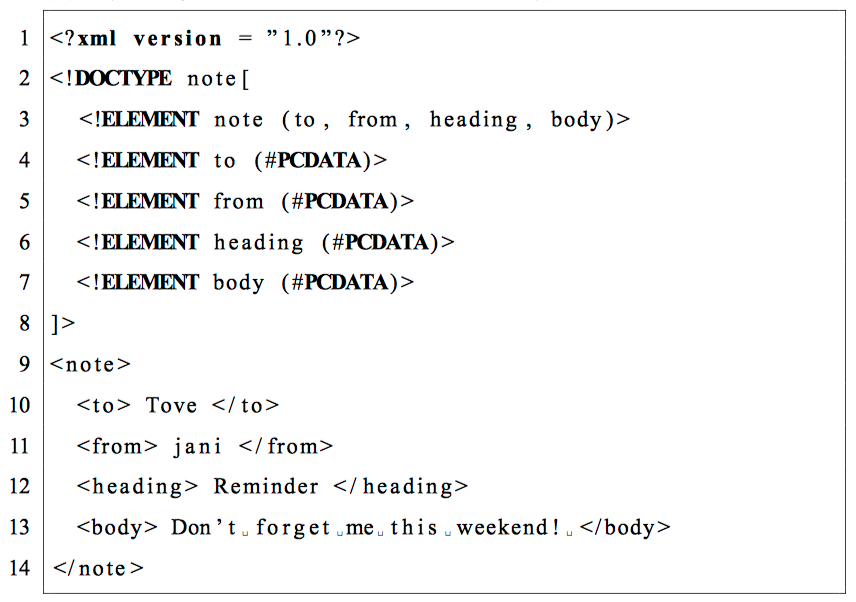
\includegraphics[scale=0.5]{xml1.png}
\caption{example1.xml}
\label{xml1}
\end{figure}

但由於XML DTD並不能完全滿足XML自動化處理的要求,也缺乏對於文件結構屬性和資料屬性的規範。所以W3C在2001年的時候提出XML Schema。XML Schema使用的語法與XML相同,且支援多種資料類型。圖\ref{xml2}是一個使用XML Schema 驗證的XML文件,在圖\ref{xml2}的第4行即宣告了XML Schema的路徑位置,而XML Schema的格式如圖\ref{schema}所示,且可以看到在語法的部分與XML相同採用巢狀的結構。而XML Schema與DTD的不同之處在第5行到第10行,XML Schema對於每一個節點有著更詳細的資料型態定義,在語法以及文件結構上面也更趨近於XML。\\\par

\begin{figure}[H]
\centering
\graphicspath{{/Users/FUDA/Documents/masterThesis/image/}}
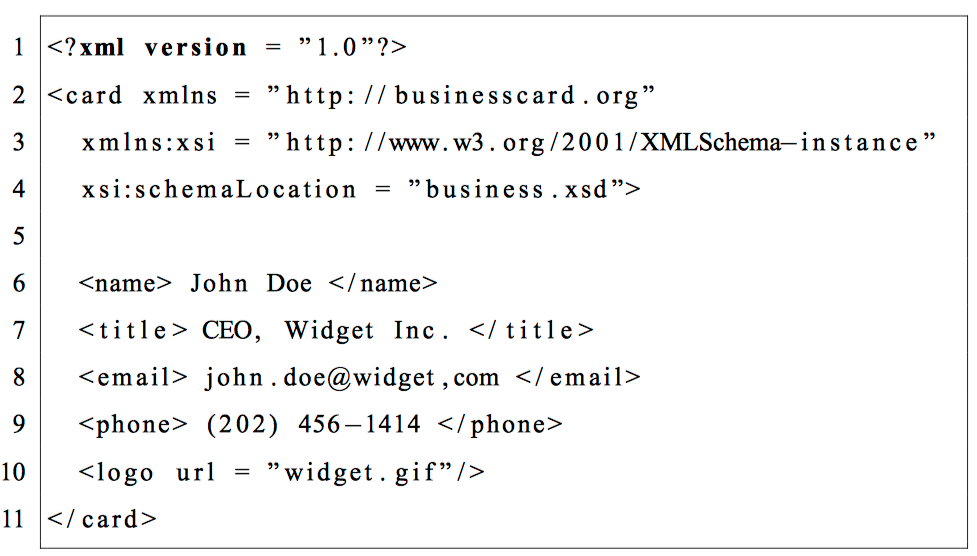
\includegraphics[scale=0.4]{xml2.png}
\caption{example2.xml}
\label{xml2}
\end{figure}

\newpage

\begin{figure}[H]
\centering
\graphicspath{{/Users/FUDA/Documents/masterThesis/image/}}
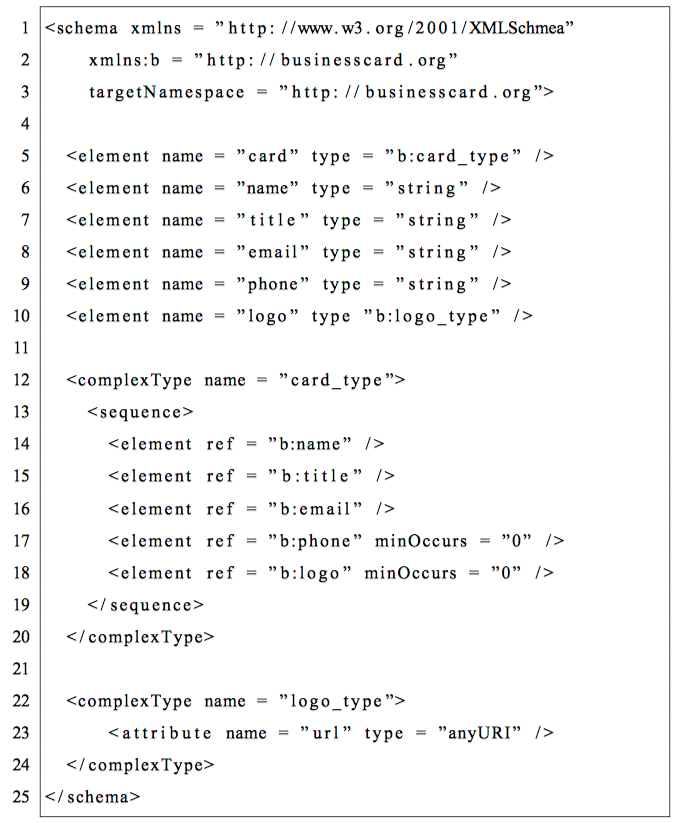
\includegraphics[scale=0.55]{schema.png}
\caption{XML Schema}
\label{schema}
\end{figure}
\newpage
\newpage
\subsection{Apache Spark}
為了解決大數據的計算問題,在2008年的時候Google提出了MapReduce\cite{mapreduce}的運算框架,用於大數據的處理。MapReduce是由Map和Reduce所組成的,Map的動作是將大的計算任務切割成小任務來操作,Reduce是將前面Map切出來並算完的小任務做合併,來取得最終的結果。後來這樣的一個計算框架演變成我們現在所熟悉的Hadoop\cite{hadoopwebsite}。\\\par
在2010年Yahoo提出了HDFS(Hadoop Distributed File System)\cite{hdfs}來解決大數據資料儲存的問題。HDFS為一個分散式檔案儲存系統,將單一檔案切割成數份,分別複製以及儲存到叢集節點當中,以達到儲存的目的。而這樣的的系統好處有三點:第一點為可擴展性(Data Scalability),當叢集的儲存空間不足的時候可以非常輕易的做擴充;第二點為容錯性(Fauit Tolerance):當其中一個儲存節點內資料有損壞的時候,系統可以從其他節點找到遺失的資料切片的備份來還原資料本身;第三點為並行性(High Concurrency):藉由分散式檔案系統可以讓資料並行處理。然而Hadoop有一個缺點,在進行MapReduce的時候,每一次的計算都是需要硬碟的I/O。這樣的行爲造成了效能的瓶頸。所以有了新一代的運算框架。\\\par
Apache Spark\cite{sparkwebsite}為一個開源的大數據分散式引擎,最初是2009年由加州大學柏克萊分校AMPLab所提出,為記憶體內(In-memory)的計算。跟Hadoop相比,Apache Spark 的計算效率比起Hadoop來說有顯著的提升,其原因為Apache Spark在運算的時候,將運算中間產生的資料暫存在記憶體中,因此可以加快整體運行速度,而Hadoop則是在每一次計算完成或是產生中間資料的時候,都必須對硬碟動作,這個動作降低了Hadoop的執行效率,而Apache Spark的設計則能夠增加計算的效率。除了上述提到的效能問題之外,Hadoop只支援Map和Reduce這兩種運算,對於現今要處理的資料來說,在撰寫程式的時候靈活度不夠,而且MapReduce在運行任務的時候,任務排程以及啟動開銷大,基於上述原因,Apache Spark是目前較好的大數據處理引擎。\\\par

Apache Spark主要的對資料的操作是使用叫做RDD(Resilient Distributed Datasets,彈性分佈資料集)\cite{zaharia2012resilient},RDD的結構如圖\ref{rdd}所示。RDD是具有容錯機制以及高效能的抽象資料結構。在圖\ref{rdd}中黃色的區塊是RDD當中所謂的Partition,是指資料的分片。一個RDD會由一個到多個的Partition所組成,程式在運行的時候,Parttion會分散至各叢集節點當中進行運算,會存放在記憶體內,所以可以快速分享各個Partition的運算結果。RDD是一個可以並列操作且有容錯機制的資料集合。且可以透過參照外部儲存系統的資料集建立,或者是透過現有的RDD轉換而創建,例如map, join, reduce等對於資料的操作,而在Apache Spark 對於RDD的操作中,有分為轉換(Transformation)和動作(Action),Apache Spark 在做資料操作的時候,採用的是惰性求值,也就是當Apache Spark 在做 Transformation的時候,並不是馬上會做資料的轉換,而是會先把要轉換的動作記錄下來,等到有呼叫Action的API的時候才會依照剛才做資料的操作並輸出結果,這樣可以使執行效能提高,例如一個資料經過 MapReduce處理後會得到一個結果,而不是返回一個大的資料集。
\begin{figure}[H]
\centering
\graphicspath{{/Users/FUDA/Documents/masterThesis/image/}}
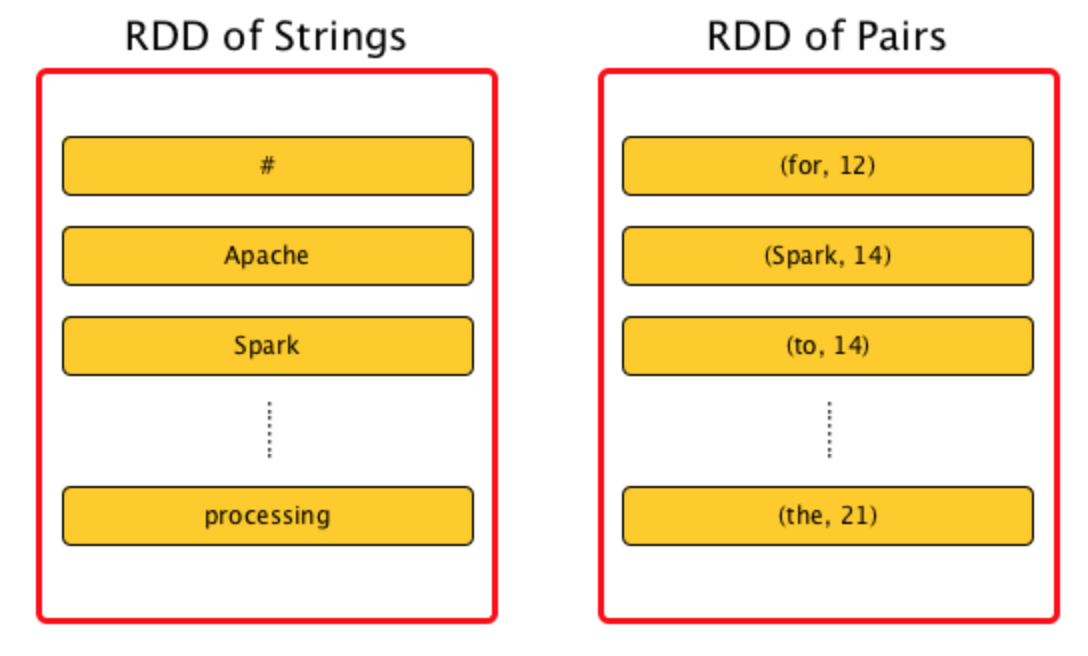
\includegraphics[scale=0.4]{RDD.png}
\caption{RDD結構}
\label{rdd}
\end{figure}

Apache Spark 有著豐富的函數庫,也針對Python, Java, Scala, R等程式語言提供一致的 API,架構如圖\ref{sparkcore},而Apache Spark 當中的核心的為Spark Core,所有API都以此為基礎。Spark Core提供了分散式任務調度、排程和基本I/O ,而主要的程式抽象化結構RDD也是定義在這邊,RDD抽象化是經由Apache Spark 所支援的程式語言整合API呈現的,簡化了寫程式的複雜性。基於Spark Core, Apache Spark 中提供了Spark SQL、Spark Streaing、MLlib以及GraphX 5大類API供使用者進行呼叫。\\\par

\begin{figure}[H]
\graphicspath{{/Users/FUDA/Documents/masterThesis/image/}}
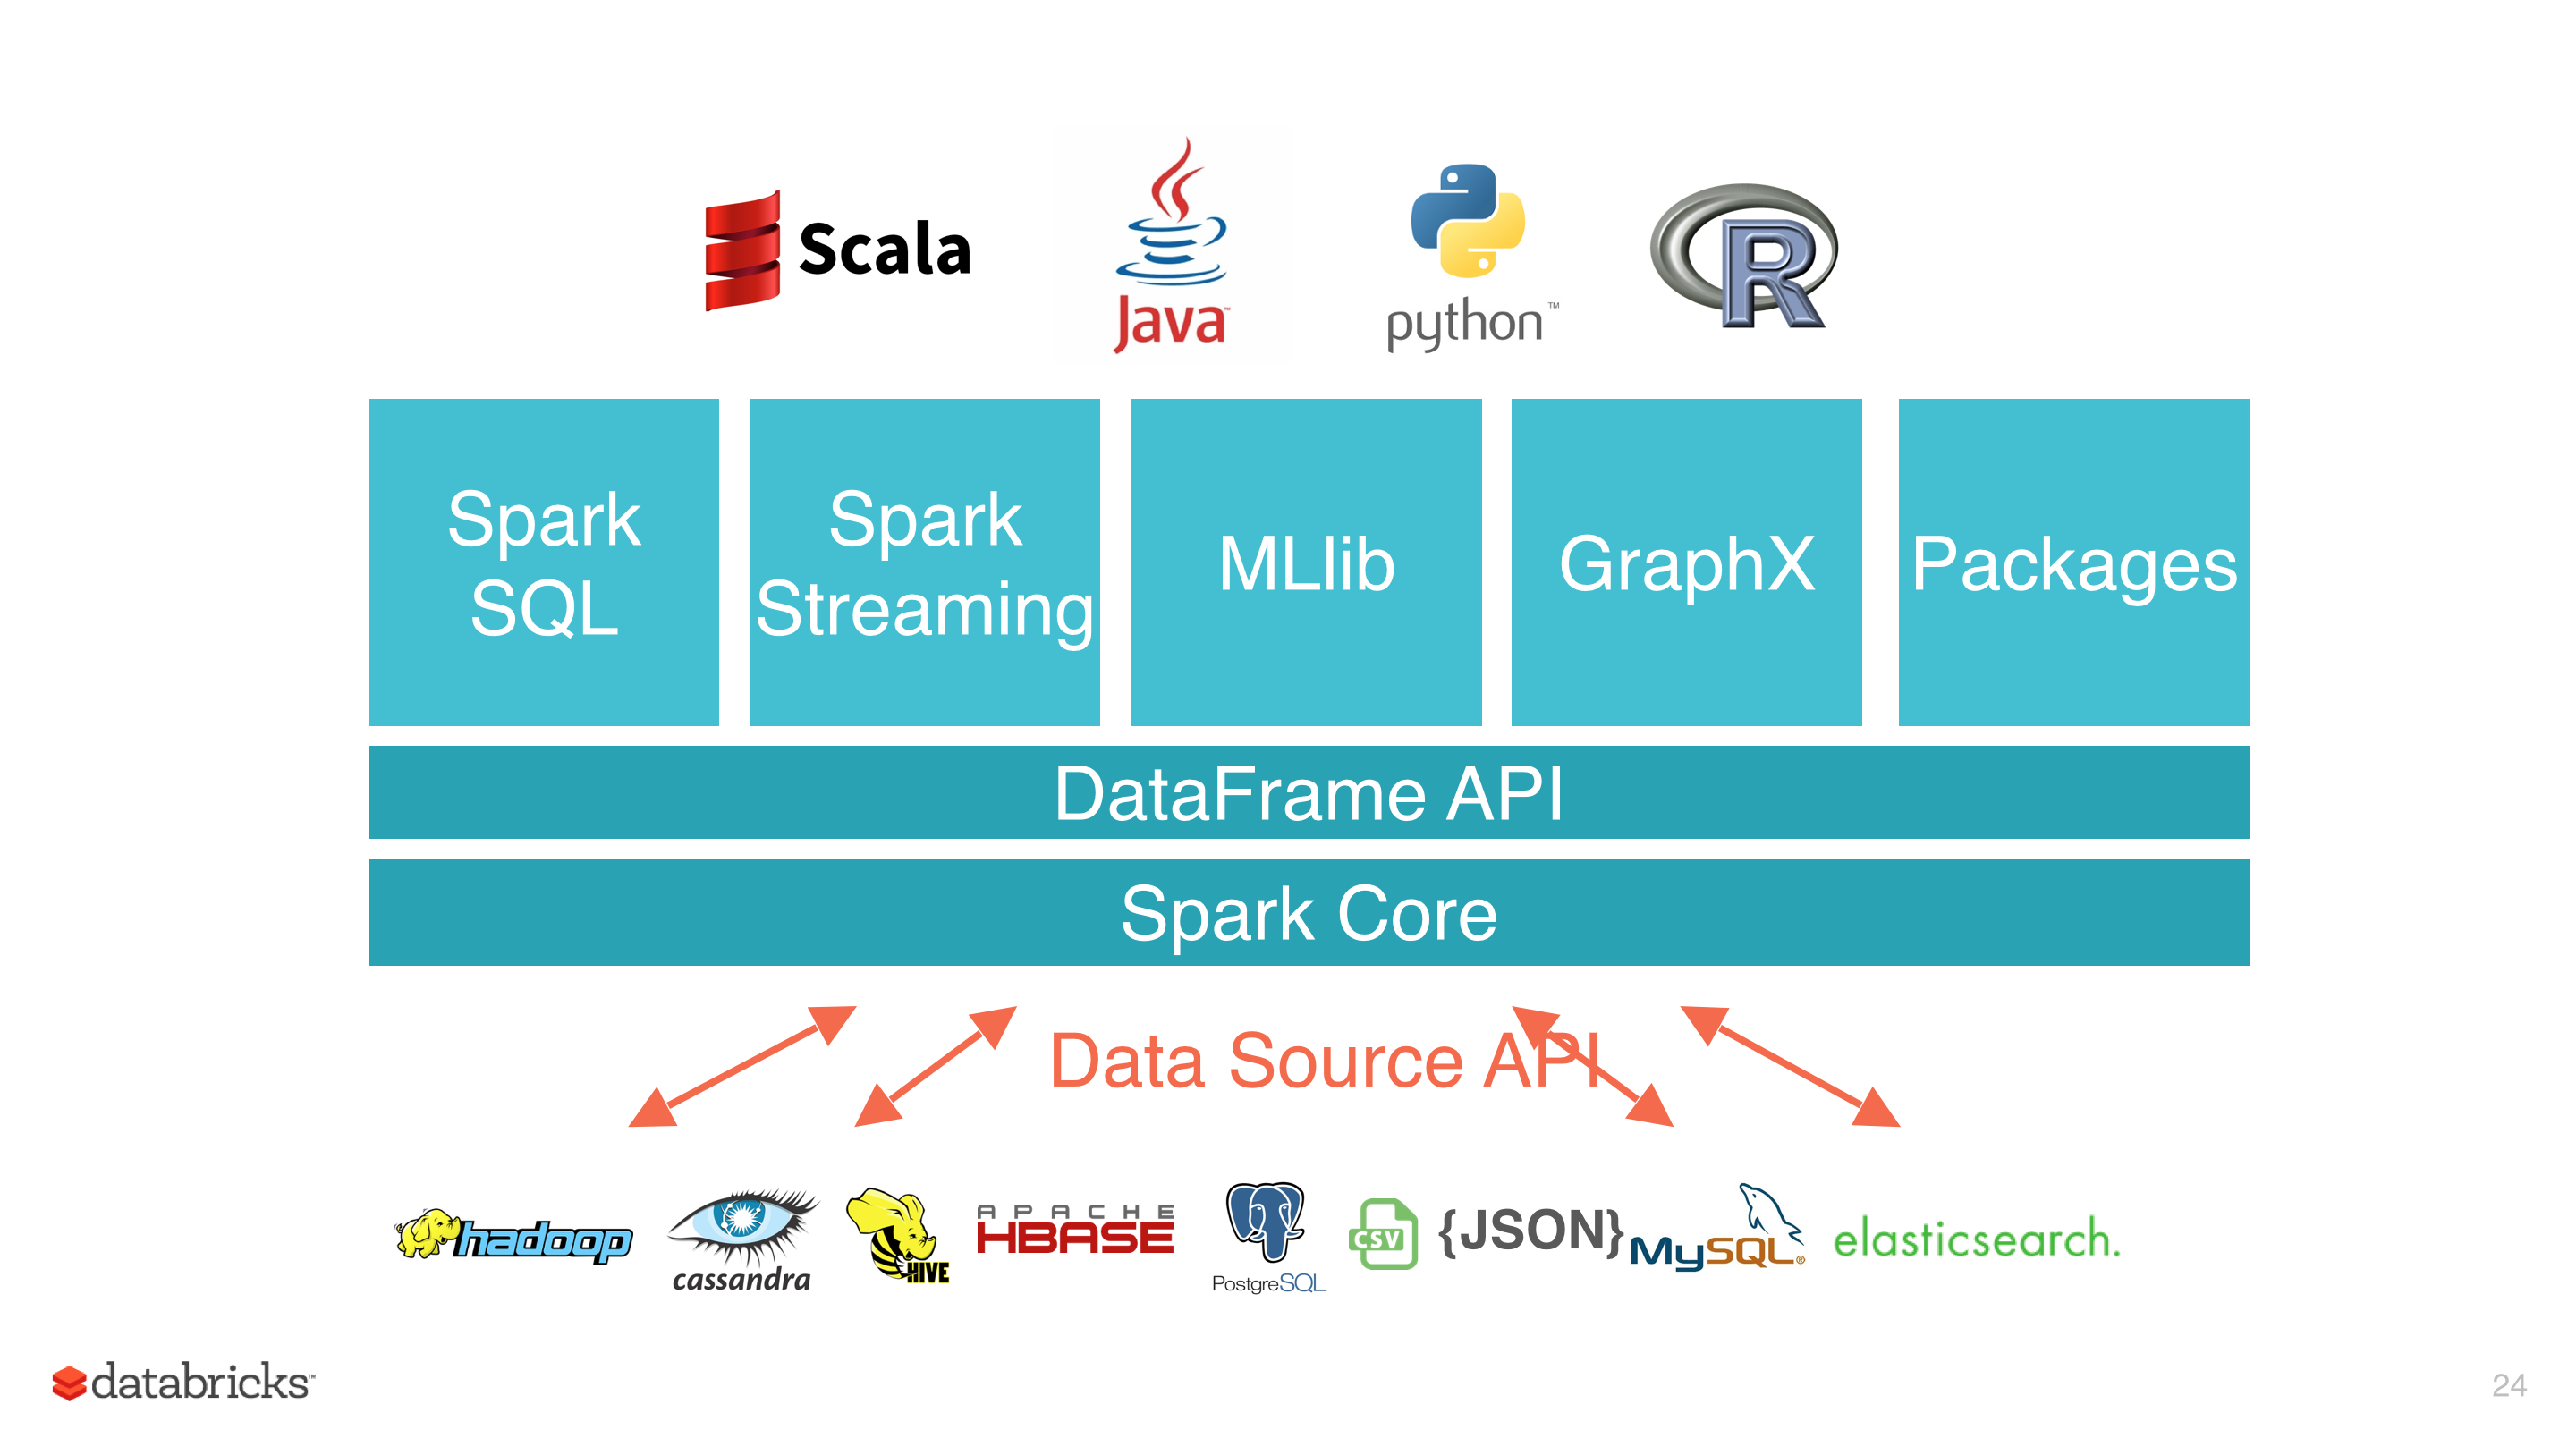
\includegraphics[scale=0.3]{spark.png}
\caption{Apache Spark 核心架構}
\label{sparkcore}
\end{figure}

Spark SQL 在Spark Core上定義了一個叫做 SchemaRDD的資料抽象化概念,提供結構化和半結構化資料的相關支援,另外Spark SQL允許使用者使用SQL遠法做資料查詢,也允許程式開發人員將SQL查詢與其他RDD所支援的資料處理方式一起使用。
Spark Streaming 是在處理即時串流資料的元件,例如web server所產生的紀錄,或是服務狀態的改變,Spark Streaming 擷取了微批次(Micro Batch)的資料並對資料執行RDD的轉換。所謂的微批次是指將每次處理時間的間隔縮小到數秒內,甚至是毫秒等級,雖然也是批次處理,但由於時間間隔變短,感覺起來會趨近於即時處理的效果。Spark Streaming的處理是針對每一個微批次做資料操作,如圖\ref{microbatch}所示:
\begin{figure}[H]
\centering
\graphicspath{{/Users/FUDA/Documents/masterThesis/image/}}
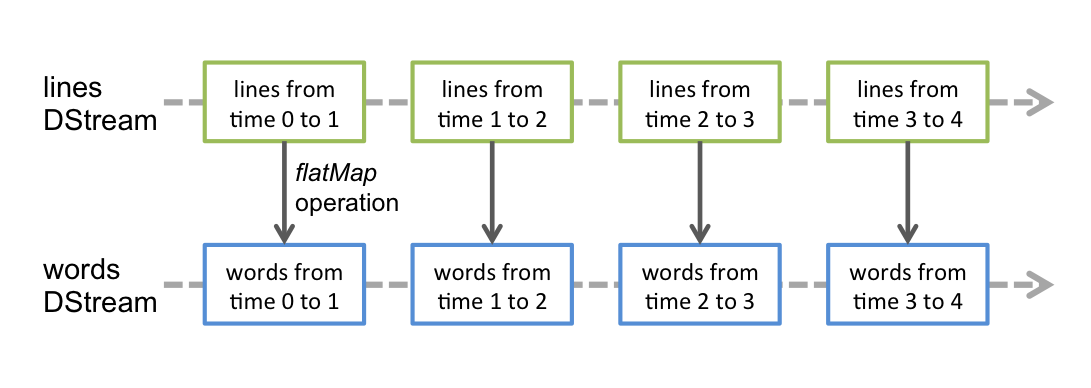
\includegraphics[scale=0.8]{streaming-dstream-ops.png}
\caption{Spark Streaming 微批次資料操作 }
\label{microbatch}
\end{figure}
MLlib是Apache Spark 所提供的機器學習(Machine Learning)函數庫,MLlib可以使用許多常見的機器學習和統計學的演算法,大幅度簡化了機器學習的時間,其中提供了匯總統計、分類、回歸、分群、協同過濾以及最佳化等機器學習及統計分析的演算法。

GraphX是Apache Spark 上的分散式圖形處理框架,此框架可用於表達圖形計算並可以類比Pregel抽象化,GraphX提供了許多處理圖像的操作,例如subgraph和mapVertices以及常見的圖形演算法。
\subsection{大數據XML文件}
所謂的大數據\cite{khan2014big}是指無法以人工管理或是處理的資料集,也可以定義為多來源的結構化或非結構化的資料,而在大數據當中,我們常常用"5V"來描述大數據的特性,這5V分別是規模性(Volume)、價值(Value)、真實性(Veracity)、時效性(Velocity)及多樣性(Variety)。\\\par
5V當中,Volume所代表的是大數據的規模,也就是大數據以傳統的儲存方式已經無法負荷此龐大的資料量或是傳統的資料處理方式已無法對其做運算了;Value是指大數據透過處理後所得到的資料產生的價值;Veracity是指資料的品質,可信度,資料是否可靠,或是結構的完整性;Velocity是指大數據資料產生的速度;Variety是指大數據的資料多樣性,在設計有關大數據的應用的時候,藉由上面五個的特性有助於檢視大數據的特徵。\\\par
XML文件的Veracity真實度這個特性是會有不同的變化的。例如XML文件如果以是否符合DTD規範, well-formed以及vaild的XML文件在真實度Veracity的特性上面就會有不同的變化。我們以兩份well-formed XML來說,上述有提到XML文件的標籤是可以讓使用者自行定義的,所以會造成兩份文件出現相同標籤名稱,意思不同,或是不同標籤名稱,意思相同的狀況,會造成不易判斷的狀況,也有可能在解析完DTD和Schema後發現兩份文件的結構很相似,所以真實度很高的狀況。\\\par
從資料理解性(data understandability)的角度詮釋Veracity的意義來看,假設有兩份XML文件,一份為基準文件B,一份為被量測文件M;我們可以從多個角度去描述「以基準文件觀之,這份被量測文件多少可能是真實的」。例如文件M與文件來源相同,因此文件M應該是真實的。或是文件M與文件B有相同的DTD,因此文件M應該是真實的。或是文件M與文件B的DataGuides相同,因此文件M應該是真實的。這些對於來源相同、DTD相同和DataGuides相同的「想法」,就是用所謂的資料理解性來描述被量測文件M是否是真實的。而由於這樣的想法可以多元且其重要性可能有差異,因此真實性就可以有程度上的區別\\\par

而在這5V當中,本研究要探討的是真實度模型在XML文件的建模與應用,在\cite{veracitymodel}有提出大數據可以由兩個面向來討論,一個是資料理解性,一個是大數據的評價基準,而本研究針對資料理解性面向進行建模,假設有n份基準XML文件以及m份被測量XML文件,使用者可以從多個角度對於XML文件進行真實度計分,XML文件真實度包含的面向極廣,對於真實度的定義每一個人不盡相同,所以本研究建構一個在Apache Spark 叢集上的Veracity真實度模型,使用物件導向程式設計(Object-Oriented Programming,簡稱OOP)的觀念,設計一個維度、屬性以及評分的抽象類別,將基本架構定義完整,做成Veracity Model API且是跑在 Apache Spark 叢集上,將實作細節交給使用者來決定,前面有提到使用者可以從不同的角度來評價XML的真實度評分,以及決定真實度要有多少維度以及多少屬性。並且本研究的模型應用在串流XML上,有別於以往傳統批次文件的處理方式,串流的資料處理方式更符合現代的資料處理架構及場景,而串流XML文件相較於傳統批次處理的XML文件處理方式又有所不同,針對一個大數據串流XML真實度評價模型是一個除了評價資料真實度之外,也可以篩選真實度較高之資料的解決方案。
\subsection{研究動機}
目前在產界與學界中,大數據已經是熱烈討論的議題,而當中的對於5V的研究也已經行之有年。本研究對於大數據的XML文件有以下分析:在Volume的部分因XML時常用於網路資料交換,而隨著大數據應用越來越多。資料交換的頻率以及資料量也會越來越大。而大量的應用也使資料產生的速度加快,是屬於Velocity的部分。資料來源多樣化以及格式上的多樣化則是屬於Variety的部分。大數據當中藏有很多隱藏資訊,藉由資料探勘等技術發現資料的隱藏價值是屬於Value的部分。最後是資料的真實度或是可信度因大數據的資料量極大,使用者或是開發者並不曉得這樣的資料是否可以使用或是否有造假資料參雜其中。\\\par

在上述5V的分析當中,Veracity是本研究關心的焦點,因為所有的資料如果真實度或是可信度不高,在儲存上因為儲存了一堆的無價值資料增加伺服器負擔,分析應用上的結果因資料是真實程度或是可信程度低所以造成結果不具任何價值。本研究將模型應用在串流XML上,以解決串流XML資料因在串流當中結構的不確定性,而導致真實度驗證困難的問題。

\subsection{論文架構}
本論文其餘架構如下。第二章相關研究將介紹XML在分散式系統的處理難處以及問題點,以及在以前是如何做真實度比較。第三章將介紹真實度模型的理論以及設計方法。第四章會實際使用物件導向設計一個真實度模型,以及介紹設計理念。第五章為使用Apache Spark 在串流XML的環境之下間模型實作至叢集當中,並且測試Apache Spark 對於模型計算是否有達到平行化以及建立Dashboard來觀察真實度模型的計算結果以及可用性。第六章將針對模型提出結語以及未來工作方向。

\newpage

\section{相關研究}
本研究建構一個在Apache Spark 叢集上的Veracity真實度模型,且應用於串流XML的真實度計算,而以往的真實度研究在大部分的文獻中都是討論文件相似度。再來XML具有樹狀結構以及自描述(self-desc特性,所以在分散式系統處理XML的時候,如何切割文件,但依然保有XML文件樹狀結構和父子節點的關係,以及在Hadoop或是Apache Spark的分散式架構下做XML的Query。本章節將就有關這些議題的文獻來做討論。
\subsection{XML文件特性}
XML結構與網頁使用的HTML十分相似,而兩者最大的不同為XML的設計為用來做資料傳輸,而HTML的設計是用來呈現資料。再者XML雖然可以自行定義Tag名稱,但有嚴格的巢狀結構規定。而HTML雖然在Tag的命名上沒有那麼自由,但有一些Tag沒有遵守巢狀結構的規定卻依然可以作動。\\\par
在\cite{w3sxml}\cite{2005xml}當中,針對XML的特性描述提到,XML可以表示成樹狀結構以及XML具有自描述(self-descriptive)的特性,以及XML可以使用如DTD或是Schema來規範其內容結構。\\\par
在自描述性中,XML可以使用標籤描述資料內容,如圖\ref{self}所示,文件裡面的Tag具有描述資料的功能,XML不負責呈現資料,所以程式開發者需要另外撰寫程式來完成。

\begin{figure}[H]
\centering
\graphicspath{{/Users/FUDA/Documents/masterThesis/image/}}
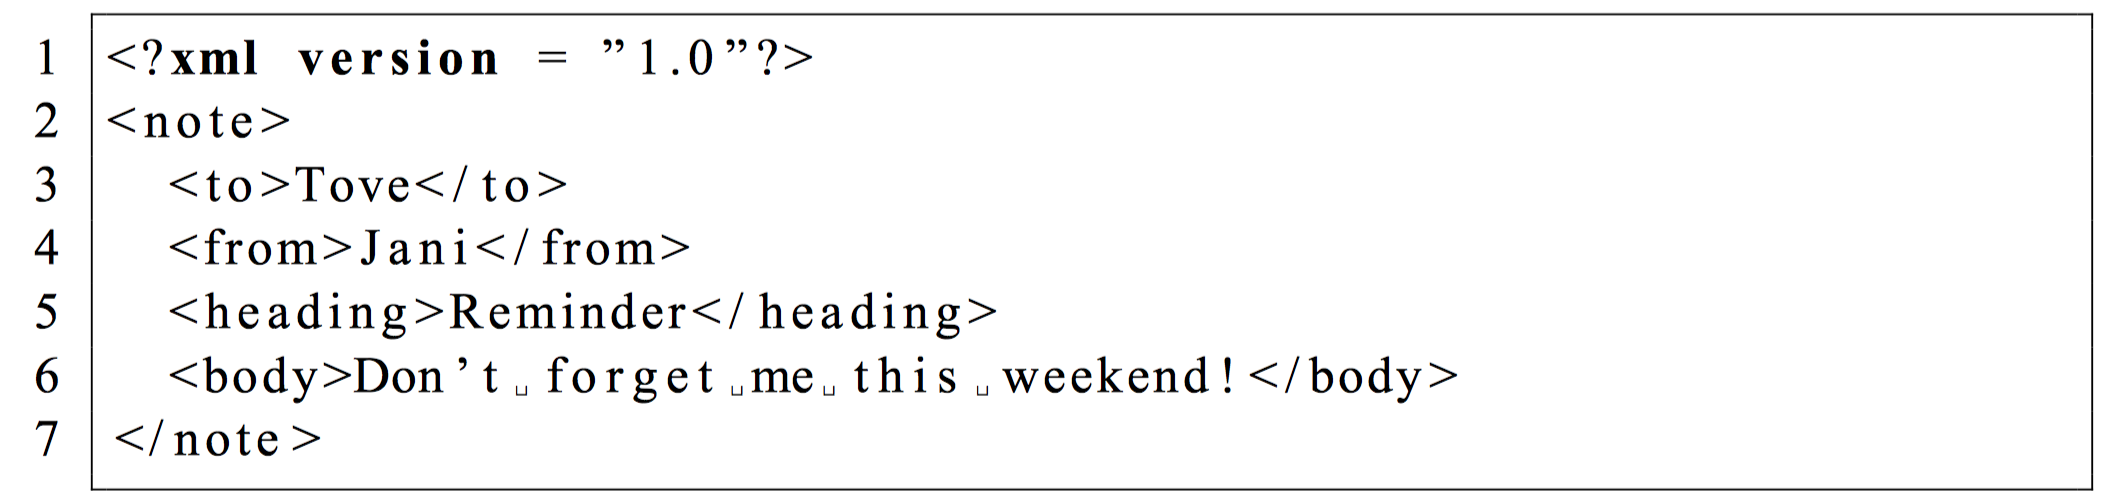
\includegraphics[scale=0.45]{xmlself.png}
\caption{XML 自描述範例}
\label{self}
\end{figure}
而XML的缺點在於需要用Tag來存放資料,以文字檔來說容量會比較大,但以現今的網路傳輸速度以及資料壓縮的技術,這也不再是問題。
\subsection{XML文件的平行化處理}
Hongjie et al.的文獻\cite{fan2018handling}提到將大型XML切割成小型的樹狀結構,存進分散式檔案系統,等到使用者的query進來之後,再將切割好的資料提取出來,使用MapReduce進行查詢。利用Hadoop的分散式系統,來到平行化query。文獻當中使用分散式檔案系統儲存XML 文件,也就是說文件在儲存之前需要經過切割。文章當中他們是採用自己設計的切割演算法,將大型XML 文件的樹狀結構切割成小型樹狀結構,接著在使用者的query進入的時候,會平行化的對這一些切割出來的小型樹狀結構作查詢。\\\par
這裡面有幾個問題點,第一點是當有多個XML文件的時候,每一份文件都會切割演算法做切割並且儲存,這時候會產生很多小文件,如何對應切割出來的小文件與原始大文件的關係,這會影響到要對哪一個文件進行處理,而文件切割和對應的部分,在\cite{eiffcientXML}當中有提到,一般在Hadoop當中,透過MapReduce切割XML文件的時候,開始標籤(<tag>)與結束標籤(</tag>)之間的關係會被切割到不同的部分,導致XML文件的節點關係不清楚,第二點是文件切割與平行化的問題,在\cite{fan2018handling}當中是使用Hadoop做處理,Hadoop 可以自行決定任務的平行化數量。而如何計算和得知切割XML的個數與平行化任務的數量各為多少是比較好的,這是在做平行化運算要面臨的問題點。\\\par

可以看到圖\ref{xmlhadoop}中紅框標示的部分即為XML文件切割完之後要進行平行化運算的部分。當中我們比較關注的是XML文件怎麼切割?被切割了幾份?以及平行畫的時候會產生的任務數量以及計算量,都是我們要考量的問題。

\begin{figure}[H]
\centering
\graphicspath{{/Users/FUDA/Documents/masterThesis/image/}}
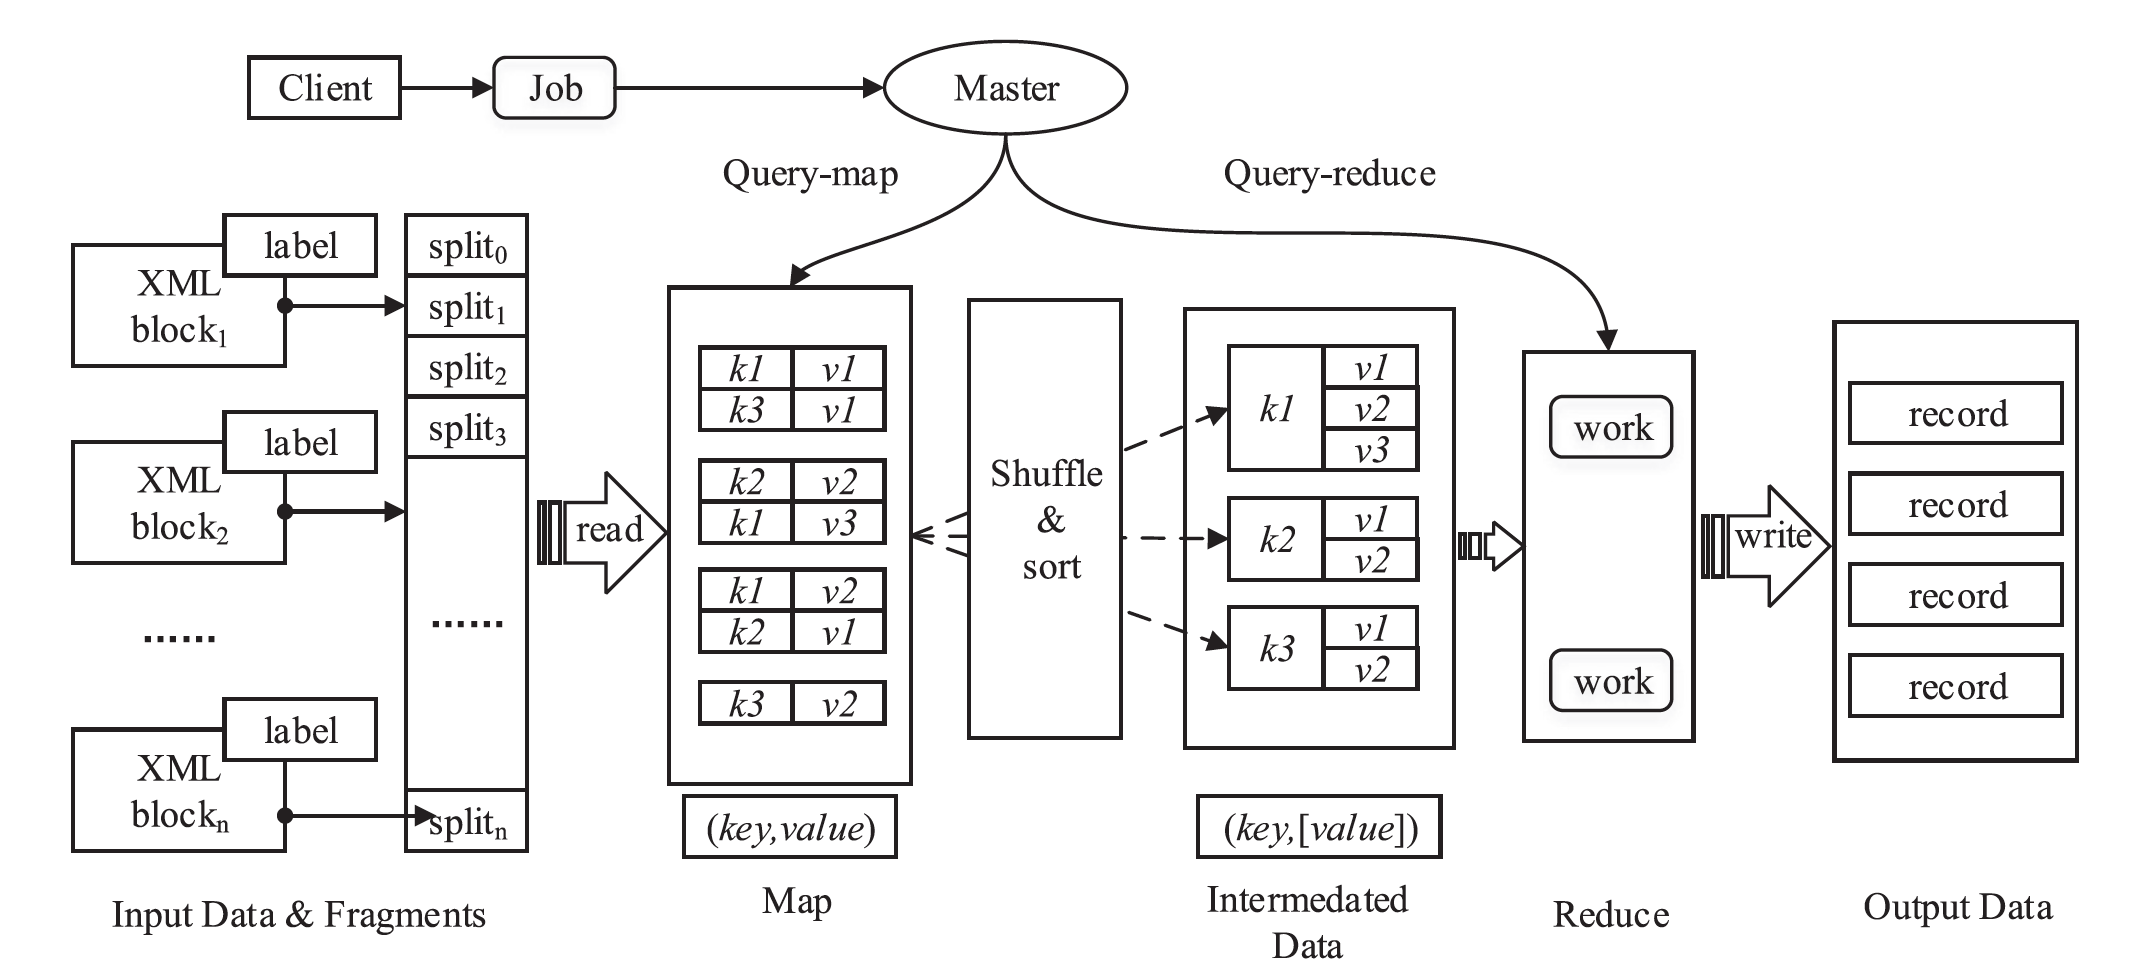
\includegraphics[scale=0.4]{xmlHadoop.png}
\caption{XML在Hadoop的切割與平行化}
\label{xmlhadoop}
\end{figure}

\subsection{XML文件相似度}
在本研究所提出的Veraicty之問題在以往的相關研究當中算少數,大部分探討是以XML文件相似度為主。在以往的研究當中會使用樹的編輯距離\cite{bille2005survey}(Edit Distance,或稱Levenshtein Distance)作相似度的比較,所謂的編輯距離為給定XML文件A與XML文件B,如果要使文件B變成跟文件A相同,需要做多少次新增、刪除以及修改的動作。在\cite{tai1979tree}當中即是採用此方法驗證兩份文件的相似度。\\\par
而在\cite{tekli2006semantic}以及\cite{tekli2012novel}當中為了增進效能,使用的是子樹(sub-tree)來做相似度的計算。而兩篇文獻不同的點在於\cite{tekli2006semantic}使用的是編輯距離,而\cite{tekli2012novel}是對於子樹的結構以及語意相似的子樹出現次數或重複次數進行計算。\cite{tekli2015approximate}則提出了基於樹編輯距離的XML語法(XML grammar)相似度驗證,並且一樣使用編輯距離來比較XML以及XML語法的相似度。\\\par
接者在\cite{algergawy2010element}當中則採用了多種的驗證方式,如Tag 名稱相似度、編輯距離、N-grams距離、Tag語意驗證等。而對於編輯距離的驗證方式除了常見的Levenshtein Distance還有使用Jaro Similarity的相似度驗證。Jaro 為兩個字串的相似度的度量,如果Jaro值越高,代表相似度越高。而另一個則為N-gram相似度,作法為將兩組欲比較之字串按照長度N切割,則可以計算兩個字串相同的子字串有多少,進而比較原字串相似度。\\\par
上述的相關研究大部分是使用編輯距離相似度演算法來做XML相似度的問題。而考量到計算效能上的問題,有幾篇的研究採用了子樹的計算來降低計算量進而強化效能。然而這樣的相似度比較對於真實度來說只是其中一個維度。而且無論是哪一種方法,在現今龐大的資料量以及串流數據的場景,皆很難完成即時性的處理。

\newpage
\newpage

\section{模型設計}

\newpage

\section{真實度模型實作}
本研究使用OOP的觀念與特性在Apache Spark上面實做真實度模型,在前面有提到對於資料的真實度評價可以從很多面向來做探討,換句話說,藉由OOP的設計方式可以讓使用者實作出真實度需要包含哪一些屬性,還有真實度的量化方法、權重加成等方法。\\\par
本研究將使用Python 作為我們設計與實作真實度模型的程式語言。原因是Python 不但是物件導向的程式語言,而且那它也是Apache Spark 所支援的程式語言。再來Python是十分易懂且容易學習的程式語言,這樣使用者在理解本模型的實作架構的時候,困難度將大大降低。\\\par
前面XML文件真實度的理論模型的描述方式是由上往下(Top-Down)的描述本研究模型的架構,而這樣描述模型的架構,在轉換成程式實作的時候,會無法使用程式語言描述清楚 ,所以在實作的時候必須採用堆疊式的方法來建構模型,也就是所謂的Bottom-Up的設計方法,本研究在設計API的時侯先將所有屬性設定完成,接著在維度陣列當中添加設計好的屬性,接著在模型陣列當中添加分類好的維度,依這樣的步驟,由下而上的把模型堆疊上去,這樣的模型是有彈性的,因為在要決定屬性隸屬於哪一個維度的時候,如果有別的模型要使用相同的屬性,那只需要把那一個屬性的物件加入到別的模型的維度陣列當中即可,這樣就可以達到相同的屬性量化方式,但是應用到不同模型維度當中,兼具了物件導向當中的彈性設計以及程式碼的重用性。
\subsection{模型實作}
真實度模型的建立,其中最重要的就是彈性以及程式的重用性,也就是用物件導向程式設計的特性來達到程式碼的重用,這在於模型是使用者決定他所認為的兩個文件真實度所具備的屬性,也就是說每個人所認為的真實度不同,在實作上就會有所不同,本研究設計真實度模型的抽象類別,首先對於XML文件真實度而言,設計一個真實度模型(Veracity Model),模型當中會具有多個維度(Dimension $D_i,  i=1\ to\ n$),在每一個維度之下會有多個屬性(Attribute $A_{i, j}, j=1\ to\ n$)來描述此維度,並且每一個維度需要有一個量化方法,對應到物件導向上可以將模型視為一個抽象類別,維度視為一個抽象類別,屬性視為一個抽象類別,所以程式上設計了 Model、Dimension、Attribute三個主要的抽象類別讓使用者去繼承並實作。\\\par
如前面提到因為一個XML文件的真實度是可以有很多面向,換言之就是可以從很多維度去探討,維度裡面會有很多屬性,這一些屬性都會有一個對於XML真實度的量化方式。\\\par
API的最上層是Model,Model底下會有真實度模型的各項元件。而Python本身沒有支援抽象類別的設計,所以要使用Python設計抽象類別就必須載入一個叫做abc的模組,並且在想要抽象的方法前面加入前綴,才能實現抽象類別的設計。整體抽象類別的設計如圖\ref{model}所示,在Model 當中 ,第7行設有dimension的list,用於建立此模型的維度,使用者必須將設計好的1到n個維度傳入這個list當中儲存,利用物件導向的特性,當Dimension的物件與Model的物件產生後,可以將多個Dimension 物件也就是多個維度使用第11行set\_dimension()的方法儲存到 dimension 這個list當中,接著在第15行設計get\_dimension()的方法來取得這個模型下的維度list。而最後需要計算模型的整體分數Veracity Value,所以在第19行設計有 veracity\_value()的方法,用以計算模型的整體分數。

\begin{figure}[H]
\centering
\graphicspath{{/Users/FUDA/Documents/masterThesis/image/}}
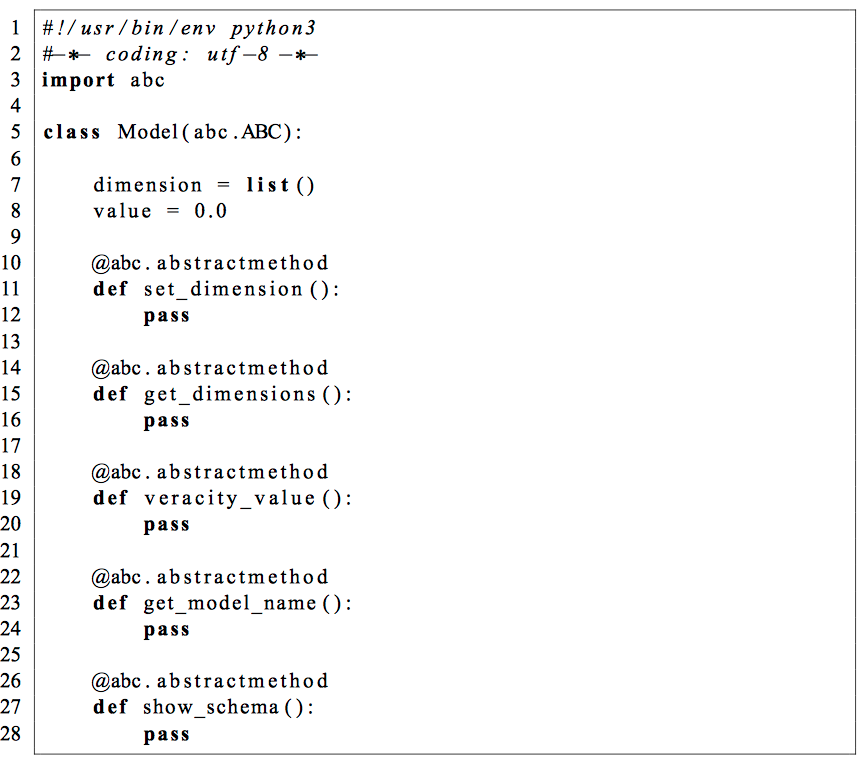
\includegraphics[scale=0.4]{model.png}
\caption{Model 抽象類別設計}
\label{model}
\end{figure}

在模型之下會有多個維度,需建立維度的類別來描述維度的架構,維度抽象類別的設計如圖\ref{dimension}所示,使用第11行set\_attributes()將建立好的屬性物件傳入attributes的 list 當中存起來,這樣就可以用物件導向的的概念去存取到下面屬性的物件的方法。另外實作上要求使用者在繼承維度的時候設定維度名稱,並且可以用第15行的get\_dimension\_name()取得維度名稱。接著需要實作第19行get\_attributes()的方法來取得先前傳入的屬性,在維度當中也會有該維度的計分,所以在第23行dimension\_degree()會設計有維度的計分方法讓使用者實作。

\begin{figure}[H]
\centering
\graphicspath{{/Users/FUDA/Documents/masterThesis/image/}}
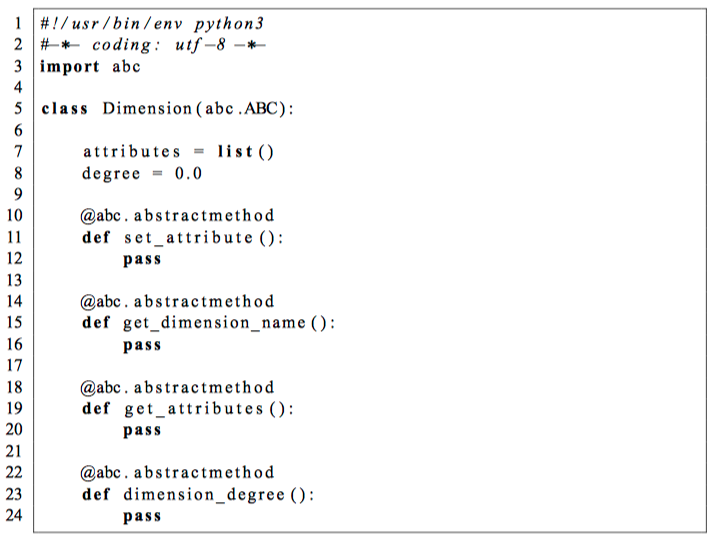
\includegraphics[scale=0.4]{dimension.png}
\caption{Dimension 抽象類別設計}
\label{dimension}
\end{figure}

而在屬性抽象類別當中,設計有兩個方法,分別是get\_attribute\_name()以及quantification(),抽象類別設計如圖\ref{attribute}所示,使用者需繼承這一個類別來實作屬性的量化方式,在get\_attribute\_name()中本實作直接設計這個方法將回傳類別名稱,也就是要求開發者在繼承並且實作的時候,類別名可以直接取成相關的屬性名稱,這樣的設計方式也是為了在存取屬性的時候方便識別。\\\par
\newpage
\begin{figure}[H]
\centering
\graphicspath{{/Users/FUDA/Documents/masterThesis/image/}}
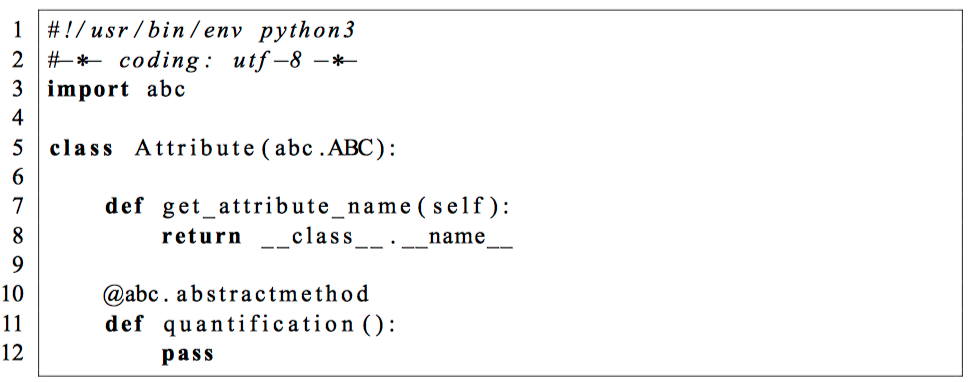
\includegraphics[scale=0.5]{attribute.png}
\caption{Attribute 抽象類別設計}
\label{attribute}
\end{figure}
以上Model、Dimension、Attribute三大類別構成了真實度模型的基礎架構,模型的建立由使用者繼承維這三大類別,使用者須先實作完屬性的量化方式接著產生屬性物件並添加至維度之內,接者再將維度物件添加至模型當中,並且在實作每一個類別的時候,須將抽象類別當中的量化方法實作完畢,接著在模型中計算總體量化的分數。\\\par
\newpage

\section{實驗}
本研究將真實度模型放在 Apache Spark 叢集當中運行,並且實際應用在串流XML文件上面。因串流資料講求即時接收即時處理,所以難在短時間內做真實度驗證。所以此模型使用在串流資料的環境下可以解決這樣的問題。本研究利用Open Data 所提供的XML自行撰寫資料產生器以及使用第三方XML文件產生器\cite{xmlgen}來產生XML文件,且每一個文件的大小皆不相同,實驗會使用客戶端程式隨機挑選文件進行上傳至串流伺服器,再由伺服器分別做資料前處理以及真實度計分,並且產生報表。\\\par
\subsection{真實度模型之串流XML文件應用架構}
本研究設計並實作真實度模型在 Apache Spark 叢集當中。Apache Spark 作為真實度計分伺服器,將接收來自客戶端傳送過來的資料,客戶端會使用 socket 將每一份XML 文件上傳至伺服器端。在Apache Spark 是使用 Spark Streaming 當中的 Socket streaming 來進行接收。而在 Socket streaming 當中會將接收到的資料進行處理,再由真實度模型進行計分,以下將針對系統當中的傳送端、處理模組以及真實度計分模組做介紹。\\\par

在資料傳送端,本研究自行實作Socket客戶端進行資料的上傳,每一個檔案會以字串的形式來做上傳,也就是說實際上客戶端發送的是持續產生的字串流,整體發送的時序圖如圖\ref{dataflow}所示:
\begin{figure}[H]
\centering
\graphicspath{{/Users/FUDA/Documents/masterThesis/image/}}
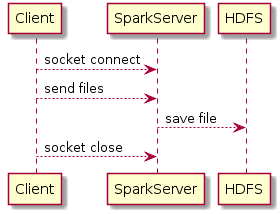
\includegraphics[scale=0.8]{dataflow.png}
\caption{資料接收與儲存流程}
\label{dataflow}
\end{figure}

在伺服器的處理模組使用的是Spark Streaming 來接收串流資料, 接收到串流資料的時候因資料是以字串流的方式發送的,所以資料處理模組會將字串流切分出每一個XML檔案,並且將處理過的資料直接送往真實度模型進行計算。資料傳送處理流程如圖\ref{recv}所示:
\begin{figure}[H]
\centering
\graphicspath{{/Users/FUDA/Documents/masterThesis/image/}}
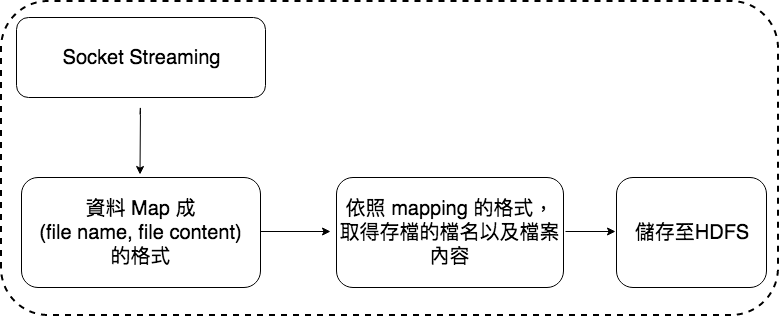
\includegraphics[scale=0.5]{recv.png}
\caption{資料傳輸處理模組}
\label{recv}
\end{figure}
資料傳送至真實度模型將傳送進來的XML文件與系統當中的基準文件做真實度計分,流程如圖\ref{process}所示:
\begin{figure}[H]
\centering
\graphicspath{{/Users/FUDA/Documents/masterThesis/image/}}
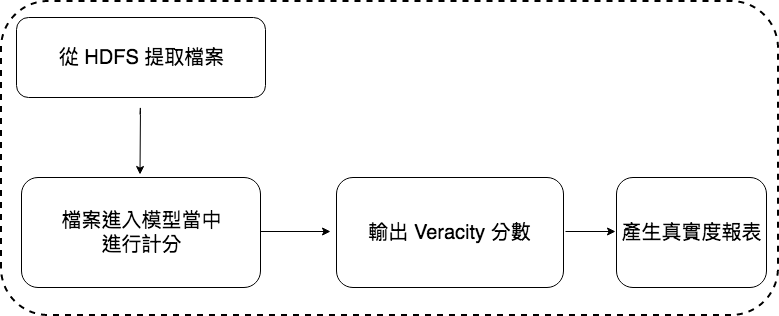
\includegraphics[scale=0.5]{process.png}
\caption{資料真實度計分模組}
\label{process}
\end{figure}

整體系統由傳送端、資料處理模組以及真實度模型計分模組所構成。利用串流做資料的上傳,從串流資料當中分割出每一個檔案來做儲存,並且使用真實度模型給予每一個檔案做真實度計分。完整系統架構如圖\ref{system}所示:
\begin{figure}[H]
\centering
\graphicspath{{/Users/FUDA/Documents/masterThesis/image/}}
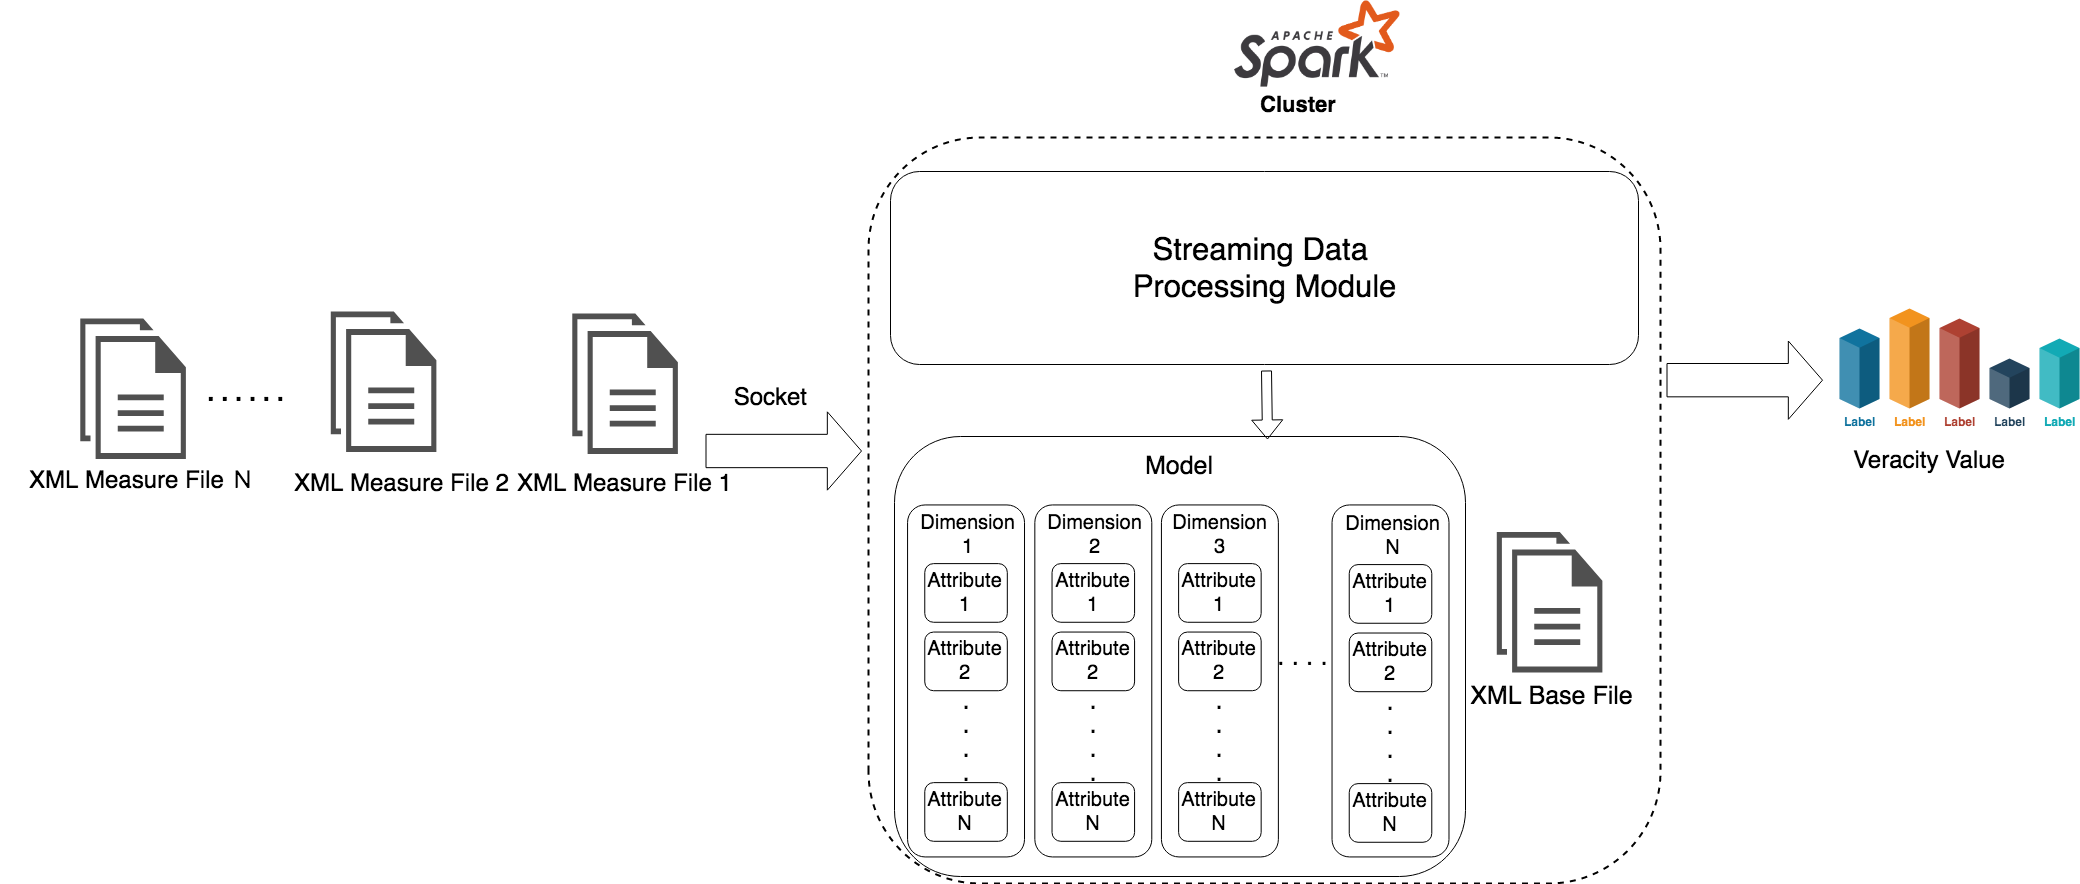
\includegraphics[scale=0.2]{streamingPro.png}
\caption{系統架構圖}
\label{system}
\end{figure}
\newpage
\subsection{真實度模型之應用實例}
本研究設計之真實度模型API應用在前面所提到的串流XML文件上,藉由實驗,驗證真實度模型應用於串流XML文件的可行性。而由於真實度的計算方式可彈性由使用者自行設計,所以根據前面的抽象類別,在真實度模型的設計應用上,本實驗設計了三個維度的真實度模型作為計算XML真實度的應用範例。\\\par
實驗設計的XML資料真實度應用範例具有三個維度,分別是文件節構、文件內容以及相似度。文件結構的維度當中有文件深度、節點數量兩個屬性,文件內容的維度當中有節點名稱以及路徑數量等兩個屬性,相似度的維度當中有路徑相似度以及節點名稱相似度兩個屬性。圖\ref{veracitymodel}為設計的模型架構:
\begin{figure}[H]
\centering
\graphicspath{{/Users/FUDA/Documents/masterThesis/image/}}
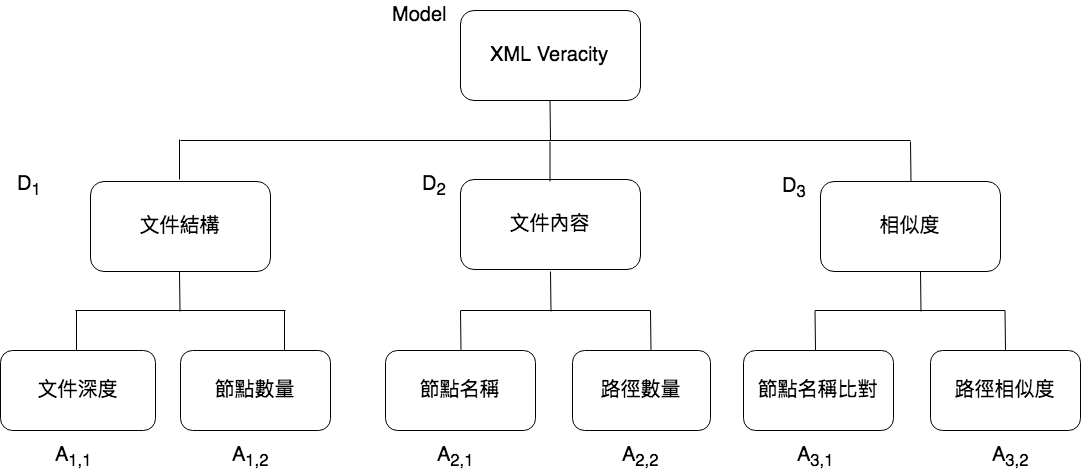
\includegraphics[scale=0.4]{xmlVeracity.png}
\caption{真實度模型}
\label{veracitymodel}
\end{figure}

這樣的架構可以對應到前面所提到的理論模型,在維度方面的定義$D_1$為XML文件結構,$D_2$為XML文件內容,$D_3$為相似度:
$$
M=\{D_1,\ D_2,\ D_3\}\\
$$
在$D_1$維度下會有2個屬性$A_{1,1}$和$A_{1,2}$,$A_{1,1}$為文件深度,$A_{1,2}$為節點數量:
$$
D_1=\{A_{1,1},\ A_{1,2}\}\\
$$
而在$D_2$維度下會有2個屬性$A_{2,1}$以及$A_{2,2}$。而屬性$A_{2,1}$代表節點名稱,$A_{2,2}$代表路徑數量:
$$
D_2=\{A_{2,1},\ A_{2,2}\}\\
$$
在$D_3$維度下有兩個屬性,$A_{3,1}$和$A_{3,2}$,分別代表節點名稱比對以及路徑相似度\cite{ristad1998learning},路徑相似度的作法是借鏡編輯距離,編輯距離會計算從字串A變成字串B需要經歷多少次的新增刪除修改,而路徑的相似度則去計算要從路徑A變成路徑B需要經歷過多次的新增刪除修改:
$$
D_3=\{A_{3,1},\ A_{3,2}\}\\
$$
理論模型確立之後,即可以依照這樣的架構來實作模型,模型建立的演算法如圖\ref{createmodel}所示:
\begin{figure}[H]
\centering
\graphicspath{{/Users/FUDA/Documents/masterThesis/image/}}
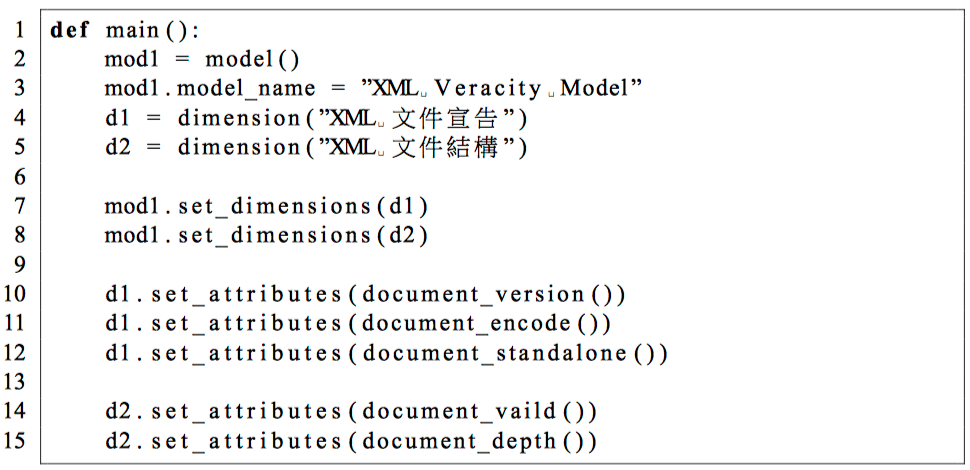
\includegraphics[scale=0.36]{createModel.png}
\caption{模型建立演算法}
\label{createmodel}
\end{figure}
接者需要設計每一個屬性的計分方式(Quantification)。而三個維度的計分方式都基於Dataguides\cite{oem}\cite{dataguides}\cite{oemweb}的結構做比較所謂的Dataguides是一種將XML的樹狀結構進行精簡化,來加速XML查詢以及節點走訪的速度,並且還可以保留各節點之間的關係。以文件結構的維度來說,下面兩個屬性:文件深度以及節點數量,在文件深度來說如果兩棵樹深度相同。在系統計分上會為滿分,如果被量測文件的樹深度與基準文件相差2以內,則分數會照著比例增加。比方說基準文件深度為5,如果被量測文件的深度為6或是4,那分數的就為加20\%。如果深度的差距到達了2層以上,系統即認為被量測文件與基準文件的資訊差異過大,所以會以比例開始扣分。在節點數量方面,如果被量測文件與基準文件的節點總數相差5個以內 ,系統會認為真實程度高,分數會較為高分。而節點數相差5個到10個以內,系統計分會偏低分。而大於10個以上則為不及格分。\\\par

在文件內容的維度來說,在節點名稱的屬性中,系統會從基準文件中隨機挑選五個節點,並且去比較在被量測文件中是否有這五個節點,有的話則依比例給分。在路徑數量的屬性中,會依照Dataguides所擷取出來的路徑數量為依據,來比較基準文件與被量測文件的路徑數量,並且依照被量測文件與基準文件的路徑數量一比例計分。\\\par

在相似度的的維度裡面,計算方法會使用常聽到的編輯距離相似度計算\cite{ristad1998learning}的方式來評分,路徑相似度的部分,系統會將基準文件與被量測文件中的最長路徑提取出來,進行編輯距離相似度比較,計算出來的相似度分數再乘上100即為屬性分數。在節點名稱比對的部分,系統會從基準文件隨機挑選五個節點,並且比較被量測文件中是否擁有這五個節點,如果有的話則依比例加分。

\subsection{實驗環境}
實驗環境是使用三台實體電腦。作業系統為Linux 發行版 Ubuntu 16.04 LTS,使用之CPU皆為8 核心,master 為16GB記憶體,兩台slave記憶體為12GB。表\ref{cluster}為機器的詳細規格。使用之Hadoop 版本為2.7,Spark版本為2.0。在HDFS中我們將每一個區塊的資料副本設置為3,軟體環境配置如表\ref{software}。
\begin{table}[H]
\begin{center}
\caption{叢集電腦規格}
\label{cluster}
\begin{tabular}{|p{3cm}<{\centering}|p{3cm}<{\centering}|p{3cm}<{\centering}|}
\hline
&Master 1台&Slave 2台\\
\hline
OS&Ubuntu 16.04 LTS&Ubuntu 16.04 LTS\\
\hline
CPU&Intel Core i7 8700@2.93GHz&Intel(R) Xeon(R) CPU E3-1230 v3 @ 3.30GHz\\
\hline
核心數&8&8\\
\hline
Memory&32 GB&12 GB\\
\hline
儲存空間&500 GB&1 TB\\
\hline
\end{tabular}
\end{center}
\end{table}

\begin{table}[H]
\caption{使用軟體版本}
\label{software}
\begin{center}
\begin{tabular}{|p{3cm}<{\centering}|p{3cm}<{\centering}|}
\hline
軟體名稱 & 版本號\\
\hline
Hadoop & 2.7版\\
\hline
Apache Spark &2.0版\\
\hline
Python & 3.6版\\
\hline
\end{tabular}
\end{center}
\end{table}

\newpage
\subsection{實驗設計}
實驗主要分成三個部分,主要的目的是要展現真實度模型的可用性以及確認在Apache Spark 中達到的平行化運算的效果。為了展現模型的效果,在第一部分的實驗中設計了一個Dashboard,用以觀察真實度模型的計分以及可視化串流文件計分的結果。第二部分則是從Apache Spark 所提供的 Web UI介面觀察資料在平行化運算的狀況,以確認對於傳流文件的處理是否有達到平行化加速的作用。第三部分的實驗將準備三種不同種類的XML文件,並且使用XML文件產生器將文件的結構做延展以及依照三種不同XML文件的規則來產生文件。在傳送的時候將三種不同種類文件混合在一起傳送,觀察真實度模型是否能正確的進行計分,並且將混合傳送的文件計算真實度並且做出三種分類。\\\par

\subsection{實驗結果}
第一部分為資料Dashboard,Dashboard的創建是使用Dash\cite{dash},Dash為一個開源的DashBoard軟體,可以自定義版面以及資料呈現方式。在Dashboard當中設計有兩個圖表,雷達圖以及表格。第一種雷達圖用來顯示真實度模型所計算出來的真實度計分,使用雷達圖上表示的面積計算出來的真實度,根據面積大小,使用者可以直接觀察到真實度的變化,Dashboard的雷達圖所呈現的真實度如圖\ref{radarchart}所示。
\begin{figure}[H]
\centering
\graphicspath{{/Users/FUDA/Documents/masterThesis/image/}}
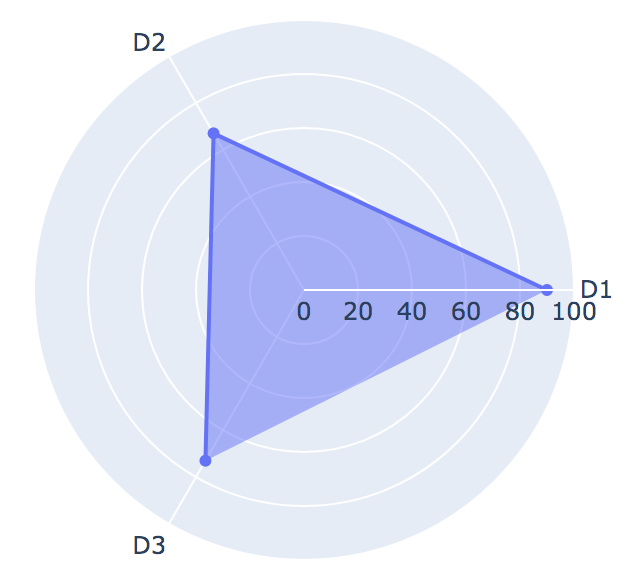
\includegraphics[scale=0.6]{radarchart.png}
\caption{真實度雷達圖}
\label{radarchart}
\end{figure}

在圖\ref{radarchart}當中,可以觀察到真實度模型的三個維度的計分。$D_1$的分數接近90分,$D_2$的分數大約為70分,$D_3$的分數約接近80。由這樣的觀察可以發現這份被量測文件的真實程度很高。\\\par
第二種表格呈現則是將真實度模型當中每一個屬性、維度以及最後的總分做完整的呈現,以補足雷達圖無法表達的細節,表格的節錄呈現如圖\ref{veracitytable}所示:
\begin{figure}[H]
\centering
\graphicspath{{/Users/FUDA/Documents/masterThesis/image/}}
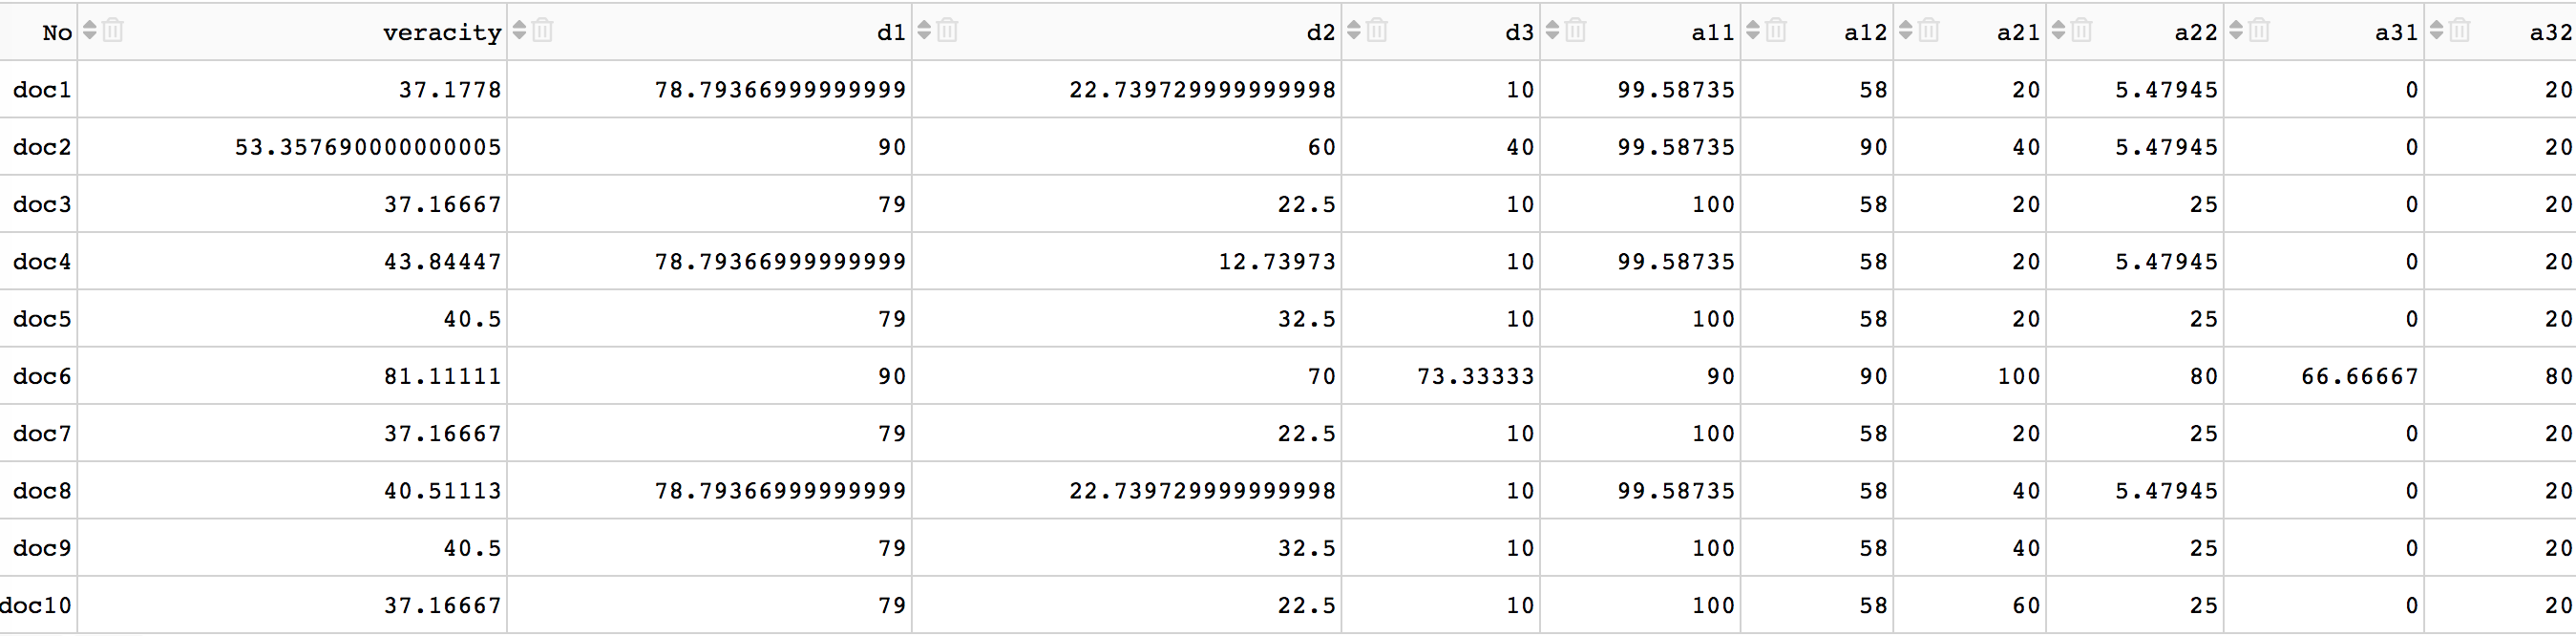
\includegraphics[scale=0.37]{veracitytable.png}
\caption{真實度表格節錄}
\label{veracitytable}
\end{figure}
在圖\ref{veracitytable}當中可以看到有著每一份被量測文件的文件編號、屬性分數、維度分數以及最後的真實度計分。在前面的雷達圖當中所呈現的是三個維度的面積,而在表格當中是呈現詳細的數據。使用者可以做交叉比對,來驗證每一份XML的真實程度。\\\par
第二部分的實驗會從Apache Spark 所提供的Web UI當中觀察串流資料的平行化,已確認串流資料的平行化。圖\ref{sparkcompute}為Apache Spark 所提供的Web UI,在當中有三列,分別代表著三台主機,而其中一欄為Active Tasks,代表說有幾幾個任務在主機上面運行,可以從圖中得知Spark driver 有將任務分發到兩台slave 去做計算,可以看到兩台slave的Active Tasks 數量都各為1,所以可以驗證平行化運算是有效的。
\begin{figure}[H]
\centering
\graphicspath{{/Users/FUDA/Documents/masterThesis/image/}}
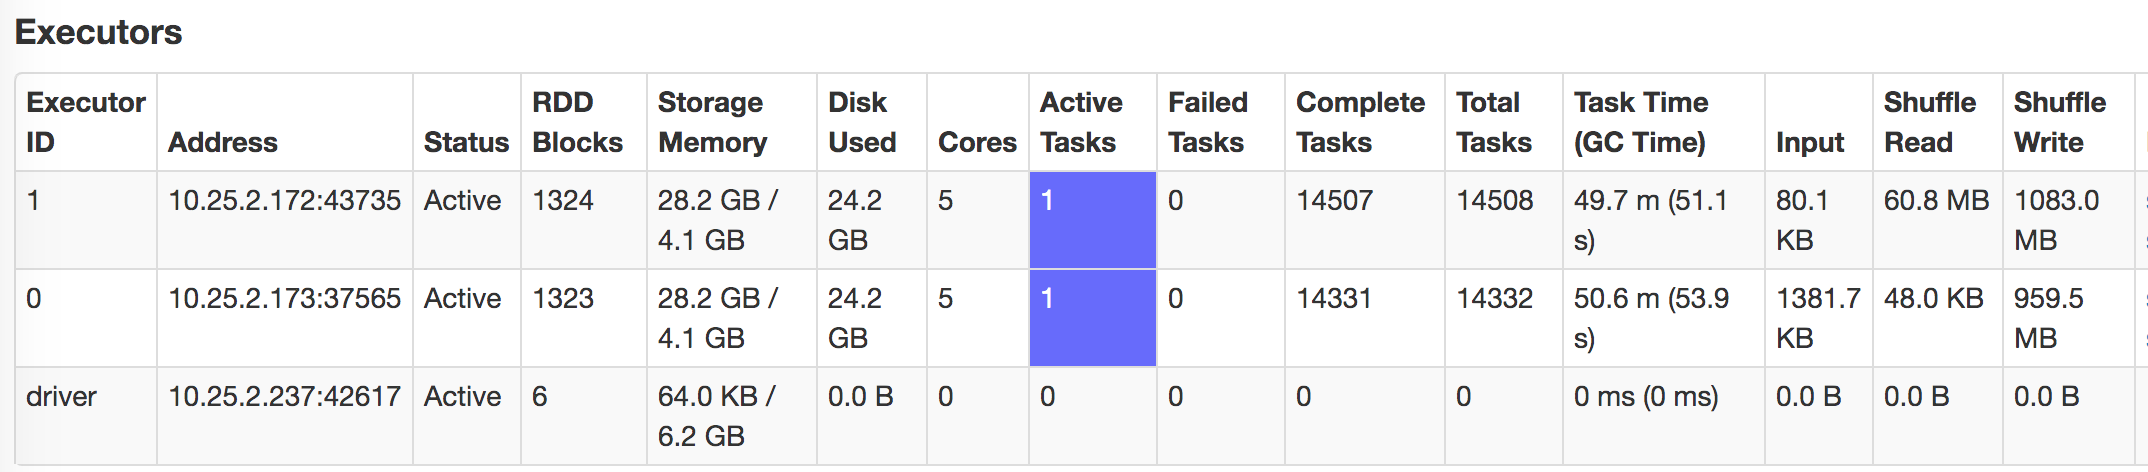
\includegraphics[scale=0.45]{sparkcompute.png}
\caption{Apache Spark 平行化}
\label{sparkcompute}
\end{figure}
最後一部分為實驗真實度模型能否將混合傳輸的資料分出不同的真實度, 實驗中準備了三種種類的XML文件,分別是美國的郵遞區號資料集\cite{usazipcode}、世界氣象的資料集\cite{worldweather}以及XML產生器所產生出來的資料集。郵遞區號的資料集Dataguides如圖\ref{zipcode.dot}所示,而世界氣象的資料集所產生出來的Dataguides如\ref{weather.dot}所示:
\begin{figure}[H]
\centering
\graphicspath{{/Users/FUDA/Documents/masterThesis/image/}}
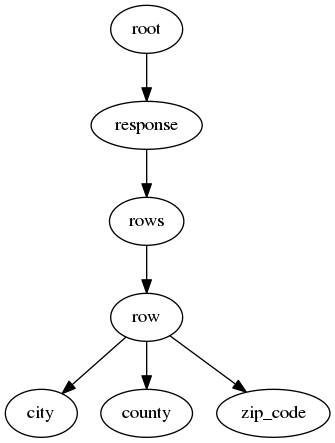
\includegraphics[scale=0.7]{zipcode.png}
\caption{郵遞區號資料集Dataguides}
\label{zipcode.dot}
\end{figure}

\begin{figure}[H]
\centering
\graphicspath{{/Users/FUDA/Documents/masterThesis/image/}}
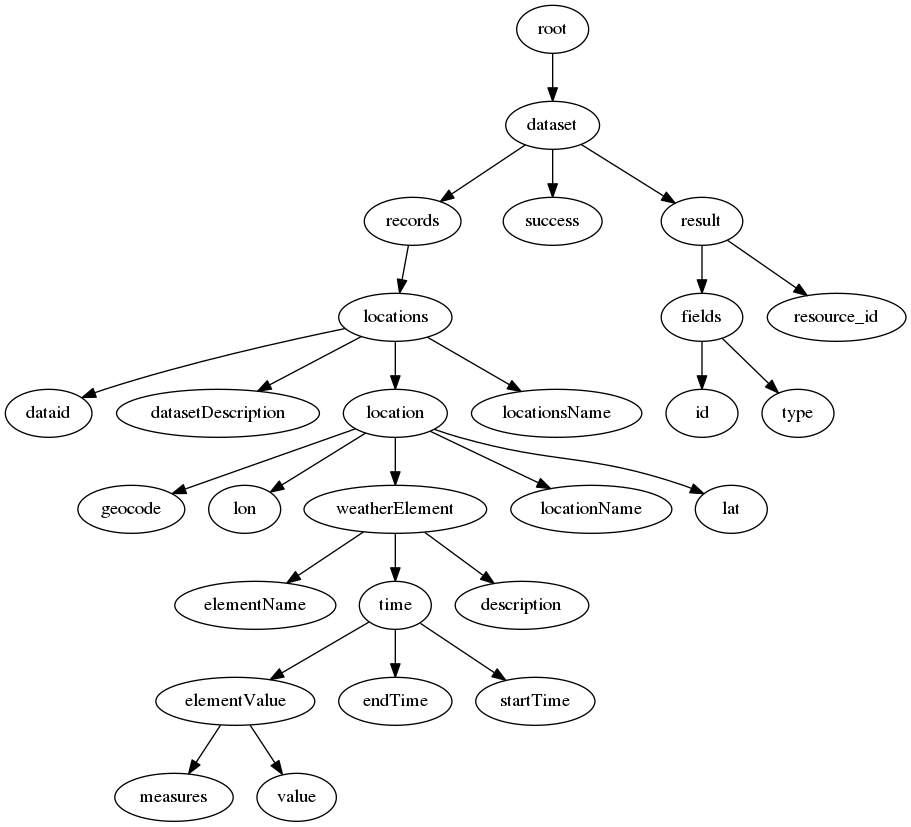
\includegraphics[scale=0.5]{weather.png}
\caption{世界天氣資料集Dataguides}
\label{weather.dot}
\end{figure}

實驗中將利用圖\ref{zipcode.dot}以及圖\ref{weather.dot}的架構撰寫文件產生器,以產生不同大小的文件來進行實驗,實驗將分成,三次實驗分別會更換三種基準文件,來測試真實度模型是否能依照基準文件來分類真實度不同的XML文件。\\\par
第一次實驗將美國郵遞區號資料集作為基準文件,第二次實驗將使用世界天氣資料集作為基準文件,第三次實驗將使用第三方XML產生器所產出的文件作為基準文件,並且比較三次實驗的平均真實度計分。\\\par

表\ref{zipbase}為第一次實驗的結果,可以從真實度計分觀察到基準文件與被量測文件同為美國郵遞區號資料集的時候,真實程度有80分以上,不同種類的資料及真實程度都明顯較低,分數都落在40分以下,可以證明模型有能力將不同種類的文件分類出來。
\begin{table}[H]
\begin{center}
\caption{基準文件為美國郵遞區號的真實度評分}
\label{zipbase}
\begin{tabular}{|p{3cm}<{\centering}|p{2.5cm}<{\centering}|p{2cm}<{\centering}|p{2cm}<{\centering}|p{2cm}<{\centering}|}
\hline
文件種類& $D_1$ &$D_2$ &$D_3$ & 真實度計分 \\
\hline
美國郵遞區號&90&78&73.33333 &80.9444438\\
\hline
世界天氣&79&29.16666667&10 &39.6582491\\
\hline
文件產生器 &78.79367&20.21486182&10&35.3597464\\
\hline
\end{tabular}
\end{center}
\end{table}
表\ref{weatherbase}為第二次實驗結果,基準文件使用世界天氣資料集,可以觀察到世界天氣的被量測文件獲得了96分,表示模型可以成功將此一種類的資料真實度分類出來。其他種類的資料真實程度也都明顯低落,分數都落在50分以下。
\begin{table}[H]
\begin{center}
\caption{基準文件為世界天氣的真實度評分}
\label{weatherbase}
\begin{tabular}{|p{3cm}<{\centering}|p{2.5cm}<{\centering}|p{2cm}<{\centering}|p{2cm}<{\centering}|p{2cm}<{\centering}|}
\hline
文件種類& $D_1$ &$D_2$ &$D_3$ & 真實度計分 \\
\hline
美國郵遞區號&74&16.7&3.125 &31.2416678\\
\hline
世界天氣&94.79&96.20625&99.03125 &96.60917\\
\hline
文件產生器&78.79367&21.18450232&9.375 &36.45106141\\
\hline
\end{tabular}
\end{center}
\end{table}
最後一個實驗的實驗結果為表\ref{docbase},基準文件為XML產生器所產生的文件,可以從表中觀察到真實度模型也可以成功將這類型的文件分類出來,並且還可以觀察到文件產生器的分數幾乎接近滿分,其原因為此類的資料是使用產生器所產生的,因為有一定的產生規則,所以導致每一份被量測文件與基準文件的差異過小,導致比對的時候真實程度差異不大。
\begin{table}[H]
\begin{center}
\caption{基準文件為文件產生器所產生之文件的真實度評分}
\label{docbase}
\begin{tabular}{|p{3cm}<{\centering}|p{2.5cm}<{\centering}|p{2cm}<{\centering}|p{2cm}<{\centering}|p{2cm}<{\centering}|}
\hline
文件種類& $D_1$ &$D_2$ &$D_3$  & 真實度計分\\
\hline
美國郵遞區號&29.13736	&3.15479&0.67568 &10.9226099	\\
\hline   
世界天氣&29.20633&13.68617273&2.02703 &14.70382\\
\hline
文件產生器&100&99.99293887&100 &99.99764629\\
\hline
\end{tabular}
\end{center}
\end{table}
綜合以上三次實驗可以觀察到三種種類的XML文件皆可以用真實度模型進行分類,其真實程度可以完全區分出三種不同的XML,從三次實驗的數據可以觀察到文件真實度分數的鑑別度,驗證了模型的可行性。
\newpage

\section{結論與未來工作}

XML在大數據的應用下做為資料交換的格式有其重要性,而資料交換的時候如何確保資料的可信度以及真實度會是一個很重要的議題。\\\par
本研究提出了基於資料理解性的真實度模型API,提出一個方式解決真實度不易表達也不易量化的問題。並且使用物件導向的觀念來設計模型,提高模型的程式重用以及程式設計彈性。並且實作範例模型放在Apache Spark叢集當中運行,以加速整體模型的處理效能。模型應用的串流XML文件,以解決串流XML資料因在串流當中結構的不確定性,而導致真實度驗證困難的問題。\\\par
本研究所提出的模型基於物件導向的設計理念,可以應用的不同的場域以及可以隨著資料特性的不同客製化出符合使用者資料特性的模型。這樣的特色可以有助於產學界降低模型的理解難度以及實作難度。\\\par
在實驗的部分,實驗中採用三種不同的資料來源,且部分資料採用自行撰寫的產生器依照資料的特性以及規則進行生成,用以驗證真實度模型之可用性。實驗數據中可以觀察到真實度模型可以將三種不同種類的資料根據基準文件成功分類出來,且符合基準文件真實度的被量測文件之真實度分數都明顯突出,驗證了模型的可用性。\\\par

本研究提出真實度模型與模型API,解決真實度不易表達也不易量化的問題,並且應用在串流XML。後續研究可以朝向平行化計算以及串流資料處理優化或是XML結構對於效能的議題上來做後續探討。
\newpage
\end{spacing}

\addcontentsline{toc}{section}{參考文獻}
\begin{center}
\renewcommand{\refname}{\textbf{參考文獻}}
\bibliographystyle{plain}
\bibliography{reference.bib}
\end{center}
\end{document}